\documentclass[12pt,a4paper]{report}

% Encoding & language
\usepackage[utf8]{inputenc}
\usepackage[T1]{fontenc}
\setcounter{secnumdepth}{3}

% Page layout
\usepackage{geometry}
\geometry{a4paper, margin=1in}
\usepackage{setspace}
\setstretch{1.5}

\usepackage{tabularx}
\usepackage{array}

% Graphics & figures
\usepackage{graphicx}
\graphicspath{{./images/}}
\usepackage{float}
\usepackage{wrapfig}

% Links & formatting
\usepackage[hidelinks]{hyperref}
\usepackage{xcolor}
\usepackage{titlesec}
\usepackage{titling}

% Math & appendix
\usepackage{amsmath}
\usepackage{appendix}

% Comments
\usepackage{comment}

\usepackage{float}
\usepackage{placeins}

% Custom section style
\titleformat{\section}
  {\normalfont\fontsize{14}{16}\bfseries}{\thesection}{1em}{}

% Paragraph indentation
\setlength{\parindent}{15pt}

% Remove page numbers for title page
\pagestyle{empty}

\begin{document}

\begin{titlepage}
    \centering
    
    \begin{minipage}{0.3\textwidth}
        \raggedright
        
\includegraphics[width=0.85\linewidth]{UAE.png}
    \end{minipage}%
    \begin{minipage}{0.4\textwidth}
        \centering
        
\includegraphics[width=0.60\linewidth]{ensah.png}
    \end{minipage}%
    \begin{minipage}{0.3\textwidth}
        \raggedleft
        
\includegraphics[width=0.75\linewidth]{dxcmaroc_logo.jpg}
    \end{minipage}
    
    \vspace*{2cm}
    
    % --- Document Type ---
    {\Large \textsc{PFA Internship Report}} \\[0.5cm]
    {\large \textbf{2\textsuperscript{nd} Year Computer Engineering}}
    
    \vspace{1cm}
    
    % --- Title Section ---
    \rule{\linewidth}{0.5mm} \\[0.6cm]
    {\LARGE \textbf{Automating the IT Service Request Lifecycle}} \\[0.3cm]
    {\Large (Request Fulfillment) Using ServiceNow} \\[0.6cm]
    \rule{\linewidth}{0.5mm}
    
    \vspace{1cm}
    
    % --- Internship Period ---
    {\large \textit{Internship Period} \\ 2 July 2026 -- 31 August 2026}
    
    \vspace{1.5cm}
    
    % --- Author & Supervisor Info ---
    % Grouping the author with the field of study and the supervisor with the company
    \begin{minipage}[t]{0.45\textwidth}
        \raggedright
        \textit{Prepared by:} \\[0.2cm]
        \textbf{Ayoub Gourstane} \\
        Computer Science Engineering
    \end{minipage}
    \hfill
    \begin{minipage}[t]{0.45\textwidth}
        \raggedleft
        \textit{Company Supervisor:} \\[0.2cm]
        \textbf{Houda AJDIR} \\
        DXC Technology Morocco
    \end{minipage}
    
    \vfill
    
    % --- Footer ---
    {\large \textbf{Academic Year: 2025--2026}}
    
\end{titlepage}
% Restore page numbering for the rest of the document
\pagestyle{plain}
\pagenumbering{arabic}

\chapter*{Acknowledgments}
\addcontentsline{toc}{chapter}{Acknowledgments}
I would like to express my sincere gratitude to the management of DXC Technology Morocco 
for giving me the opportunity to complete my PFA internship remotely and to contribute
to a professional project within a real working environment. This experience allowed me to put 
the knowledge acquired during my studies into practice while developing new technical and professional skills.

I would especially like to thank Houda AJDIR, my company supervisor, for her guidance, availability,
and continuous support throughout the internship. Despite the remote nature of the internship, her explanations, 
feedback, and technical guidance were essential to understanding the project requirements, addressing the challenges 
encountered, and progressing effectively throughout the different stages of the work.

The remote nature of the internship also encouraged me to work independently, organize my tasks effectively, 
manage my time, and take responsibility for the progress of my work. I am grateful to my supervisor for the trust 
and autonomy given to me throughout this experience.

Finally, I would like to thank everyone who contributed, directly or indirectly, to the success 
of this internship and to the completion of  this report.

This internship has been a valuable step in my academic and professional development, 
and I am grateful for the opportunity and experience it provided me.


\chapter*{Abstract}
\addcontentsline{toc}{chapter}{Abstract}
This report presents the work carried out during my PFA internship at \textbf{DXC Technology Morocco}.
The internship was conducted remotely and was divided into two main phases. The first month was dedicated
to professional training through a ServiceNow System Administrator course, which provided me with 
the fundamental knowledge required to understand and work with the ServiceNow platform. 
The second month focused on applying this knowledge through the design and implementation of 
a Service Request Fulfillment solution.

The project aimed to structure and automate the management of IT service requests in order to improve 
their processing, traceability, assignment, and overall fulfillment. Several service catalog items
were designed and configured, including User Account Creation, Enterprise VPN Access, Software Installation, 
IT Hardware Requests, and Password Reset. The implementation involved defining request forms, approval processes, 
fulfillment tasks, assignment rules, notifications, and automated closure. 
Service Level Agreements (SLAs) were also configured to support service monitoring and ensure compliance with defined service targets.

The project was developed within the ServiceNow environment through a structured process involving requirements 
analysis, configuration, testing, validation, and deployment preparation. This internship provided me 
with practical experience in ServiceNow administration and configuration, IT Service Management, workflow automation, and 
requirements analysis. It also strengthened my ability to work independently, manage my time effectively, 
and apply newly acquired technical knowledge to a practical professional project.

\noindent\textbf{Keywords:} ServiceNow, IT Service Management (ITSM), Service Request Fulfillment, Service Catalog, Workflow Automation, Service Level Agreement (SLA), Business Rules

\chapter*{List of abbreviations}
\addcontentsline{toc}{chapter}{List of abbreviations}
\begin{tabular}{|l|l|}
\hline
\textbf{abbreviation} & \textbf{Meaning} \\
\hline
IT  & Information Technology \\
\hline
ITSM  & Information Technology Service Management \\
\hline
ITIL  & Information Technology Infrastructure Library\\
\hline
UI  & User Interface \\
\hline
SLA  & Service Level Agreement \\
\hline
aPaaS  & Application Platform as a Service \\
\hline
SaaS  & Software as a Service \\
\hline
UAT  & User Acceptance Testing \\
\hline
CMDB  & Configuration Management Database \\
\hline
\end{tabular}

\tableofcontents

\listoffigures

\listoftables

\chapter{General Context of the Internship}

\section{Introduction}
this chapter presents the general context of my PFA Internship at \textbf{DXC Technology Morocco}. 
It begins with an overview of the host organization and its activities, followed by a presentation 
of the internship context and working environment. The chapter then introduces the main project 
carried out during the internship, including its background, problem statement, objectives, and 
scope. Finally, the methodology and general approach adopted throughout the project are presented.

\section{Presentation of the Host Organization}

\subsection{DXC Technology Worldwide}
DXC Technology is a global technology services company that helps organizations
manage, modernize, and transform their information technology environments. The
company provides a broad range of IT services and solutions covering applications,
cloud and infrastructure, cybersecurity, analytics, workplace services, and business
process services.

DXC Technology serves organizations across multiple industries and geographical
regions, supporting them in addressing complex technological and operational
challenges. Its activities combine consulting, technology implementation, systems
integration, and managed services to support the transformation and continuous
operation of enterprise IT environments.

\begin{figure}[H]
    \centering
    
\includegraphics[width=0.2\textwidth]{dxcmaroc_logo.jpg}
    \caption{DXC Technology Logo}
    \label{fig:dxc-logo}
\end{figure}

\subsubsection{Computer Sciences Corporation (CSC)}

Computer Sciences Corporation (CSC) was an American information technology
company specializing in technology consulting, systems integration, outsourcing,
and IT services. Founded in 1959, CSC developed extensive expertise in helping
organizations design, implement, and manage complex information systems.

Over the years, CSC established an international presence and provided technology
services to organizations across various industries. Its experience in consulting,
application services, and enterprise IT management later became an important part
of the capabilities brought together within DXC Technology.

\begin{figure}[htbp]
    \centering
    
\includegraphics[width=0.3\textwidth]{csc_logo.png} 
    \caption{CSC logo}
    \label{fig:csc-logo}
\end{figure}


\subsubsection{Hewlett Packard Enterprise (HPE)}

Hewlett Packard Enterprise (HPE) is an American technology company focused on
enterprise computing, infrastructure, networking, storage, and related IT
services. HPE was established in 2015 following the separation of Hewlett-Packard
Company into two independent organizations.

The Enterprise Services business of HPE provided organizations with services
related to infrastructure management, outsourcing, applications, and enterprise
technology environments. This business subsequently became one of the two major
components involved in the creation of DXC Technology.

\begin{figure}[htbp]
    \centering
    
\includegraphics[width=0.3\textwidth]{hpe_logo.png} 
    \caption{HPE logo}
    \label{fig:hpe-logo}\textsc{}
\end{figure}

\subsubsection{Creation of DXC Technology}

DXC Technology was created in 2017 through the merger of Computer Sciences
Corporation (CSC) and the Enterprise Services business of Hewlett Packard
Enterprise (HPE). The merger combined the technological expertise, service
capabilities, and international presence of both organizations to establish a
new global IT services company.

DXC Technology officially began operations on April 1, 2017. Since its creation,
the company has continued to develop its expertise in areas such as applications,
cloud and infrastructure, cybersecurity, analytics, workplace services, and
business process services.

\begin{figure}[htbp]
    \centering
    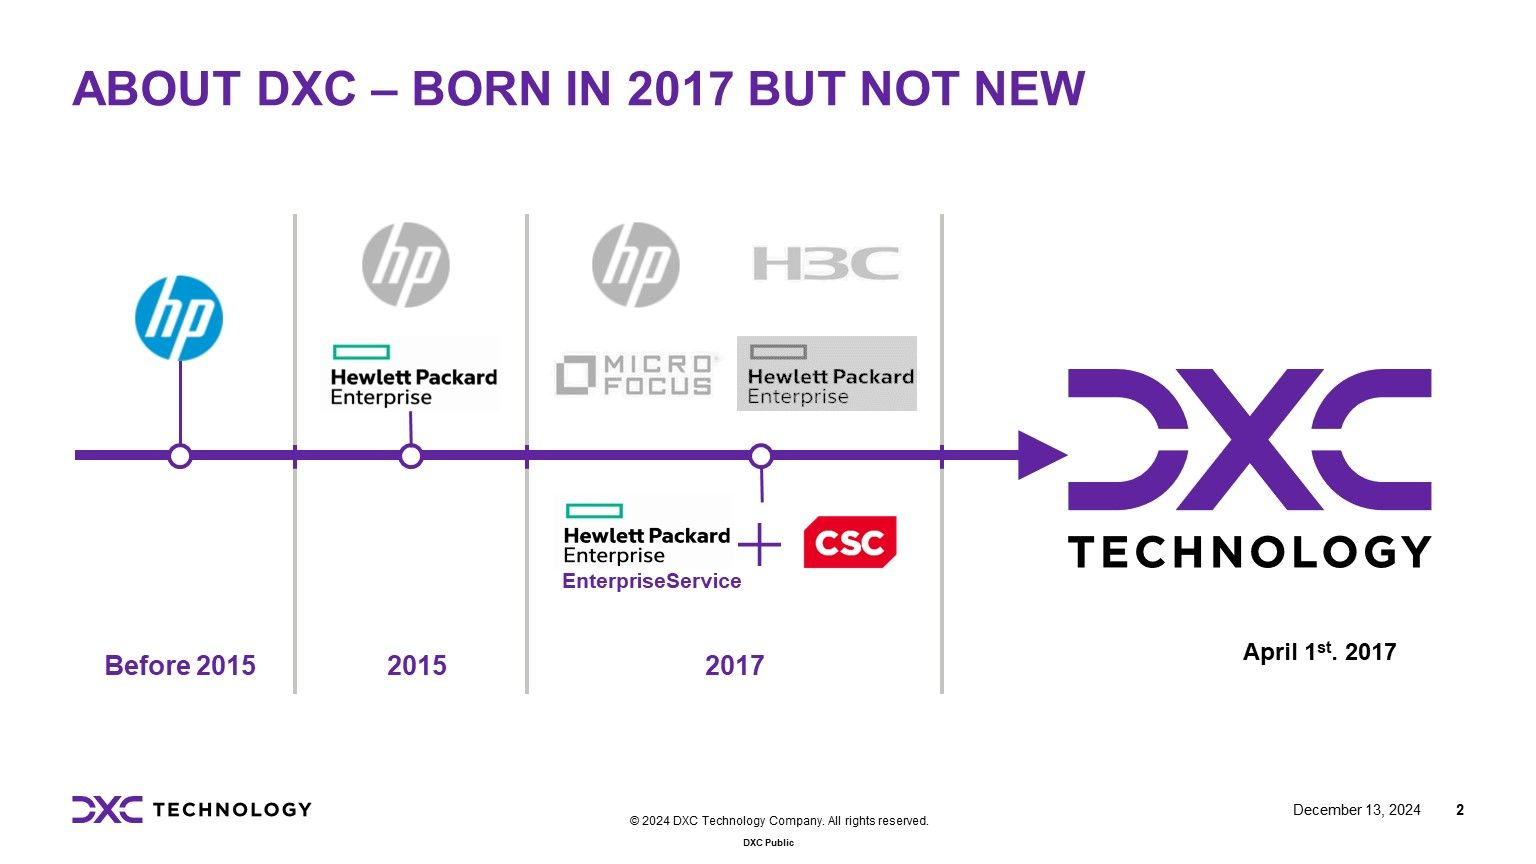
\includegraphics[width=0.9\textwidth]{dxc_timeline.jpg}
    \caption{Evolution leading to the creation of DXC Technology}
    \label{fig:dxc-history}
\end{figure}


\subsection{DXC Technology Morocco}

DXC Technology Morocco is the Moroccan entity of DXC Technology and operates
within the company's global network of technology services. The organization
supports major public and private-sector organizations in their digital
transformation initiatives and provides a range of technology and business
services.

\subsubsection{Overview of DXC Technology Morocco}

\begin{table}[H]
    \centering
    \begin{tabular}{|l|l|}
        \hline
        \textbf{Item} & \textbf{Information} \\ \hline
        Company & DXC Technology Morocco \\ \hline
        Location & Technopolis, Rabat, Morocco \\ \hline
        Established & 2007 \\ \hline
        Current name & DXC Technology Morocco since 2017 \\ \hline
        Parent organization & DXC Technology \\ \hline
        Local partner & Caisse de Dépôt et de Gestion (CDG) \\ \hline
        Main activity & Information Technology Services \\ \hline
    \end{tabular}
    \caption{DXC Technology Morocco at a Glance}
    \label{tab:dxc-morocco}
\end{table}

\subsubsection{History of DXC Technology Morocco}

The history of DXC Technology Morocco dates back to 2007, when the Moroccan
entity was established through a partnership between Electronic Data Systems
(EDS) and the Caisse de Dépôt et de Gestion (CDG). The organization initially
operated from a 450~m$^2$ site with 36 employees and began providing IT services
to support CDG's activities.

In August 2008, EDS was acquired by Hewlett-Packard (HP), marking an important
step in the development of the Moroccan entity. In 2009, the organization
integrated HP's activities and changed its branding to HP CDG IT Services Maroc.
During the same period, it obtained ISO 9001 certification.

The organization continued to expand during the following years. In 2011, it
was recognized as the fifth-best employer. In 2012, the organization moved to a
new site designed to accommodate up to 1,000 employees and was recognized as the
third-best employer. By 2014, it had reached the second position in the
best-employer ranking.

These milestones illustrate the progressive development of the Moroccan
organization in terms of infrastructure, workforce, and recognition as an
employer.

\begin{figure}[H]
    \centering
    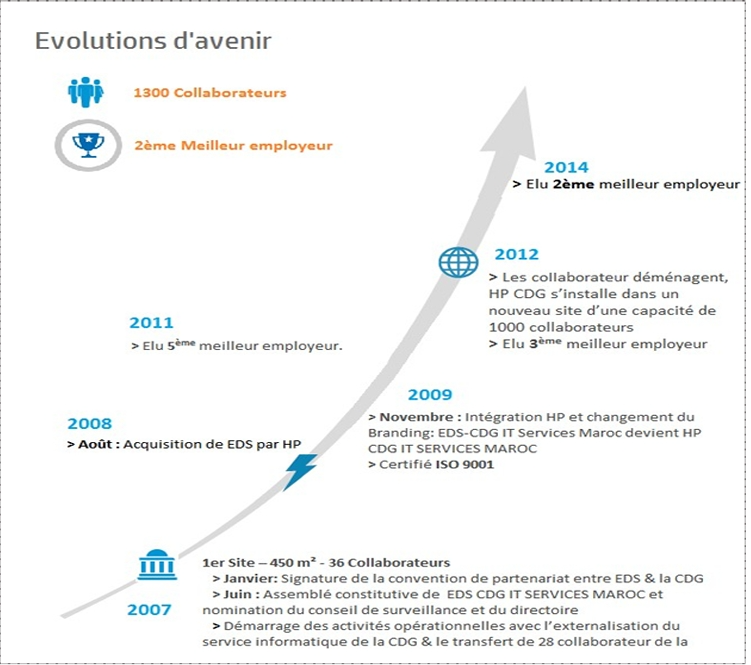
\includegraphics[width=0.8\textwidth]{dxc_morocco_history.png}
    \caption{Historical development of DXC Technology Morocco}
    \label{fig:dxc-morocco-history}
\end{figure}

Following these developments, the organization underwent another major
transformation in 2017 following the global creation of DXC Technology through
the combination of Computer Sciences Corporation (CSC) and Hewlett Packard
Enterprise's Enterprise Services business. The Moroccan entity subsequently
adopted the DXC Technology name, becoming part of DXC Technology's global
organization.

\subsubsection{DXC Technology Success Story}
The following figure presents the success story of DXC Technology and the evolution of the number of employees since 2007.

\begin{figure}[H]
    \centering
    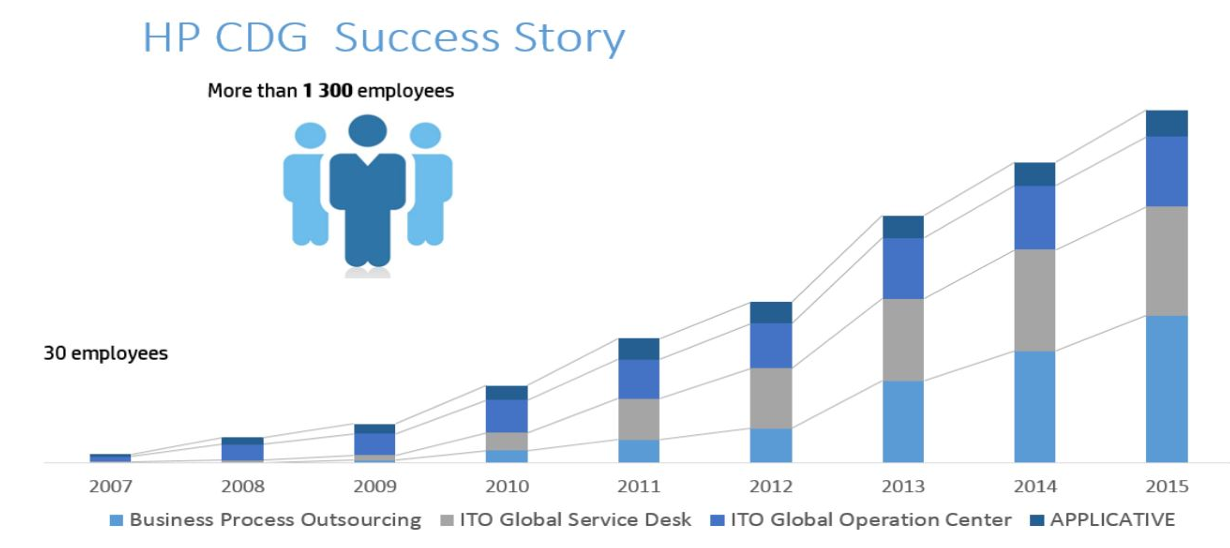
\includegraphics[width=0.8\textwidth]{success_history.png}
    \caption{DXC Technology Success Story}
    \label{fig:success-history}
\end{figure}

\subsubsection{Business Areas and Services}

DXC Technology Morocco provides a diversified range of technical and functional
services organized around several major areas of expertise. These areas combine
technology capabilities with business-oriented services to address the
requirements of organizations across different sectors.

\begin{itemize}
    \item \textbf{Data Center:} Hosting, technical support, infrastructure
    supervision, and deployment of cloud solutions for efficient data management.

    \item \textbf{Cloud Infrastructure:} Design and modernization of hybrid
    cloud environments and migration of traditional platforms toward evolving
    cloud architectures.

    \item \textbf{Applications:} Integration, migration, modernization, and
    maintenance of enterprise applications.

    \item \textbf{ServiceNow:} Integration, customization, and optimization of
    business and IT processes through the ServiceNow platform, particularly in
    areas such as IT Service Management (ITSM) and IT Operations Management (ITOM).

    \item \textbf{Workplace and Mobility:} Secure access to enterprise resources
    through endpoint management, device management, and workplace virtualization
    solutions.

    \item \textbf{Business Process Services:} Management and support of business
    processes, including customer service and automated request processing.

    \item \textbf{Cybersecurity:} Security assessment, risk management,
    monitoring, incident management, and deployment of security solutions.

    \item \textbf{Business Intelligence and Analytics:} Development of analytical
    platforms and data solutions to support reporting, analysis, and
    decision-making.
\end{itemize}

\begin{figure}[H]
    \centering
    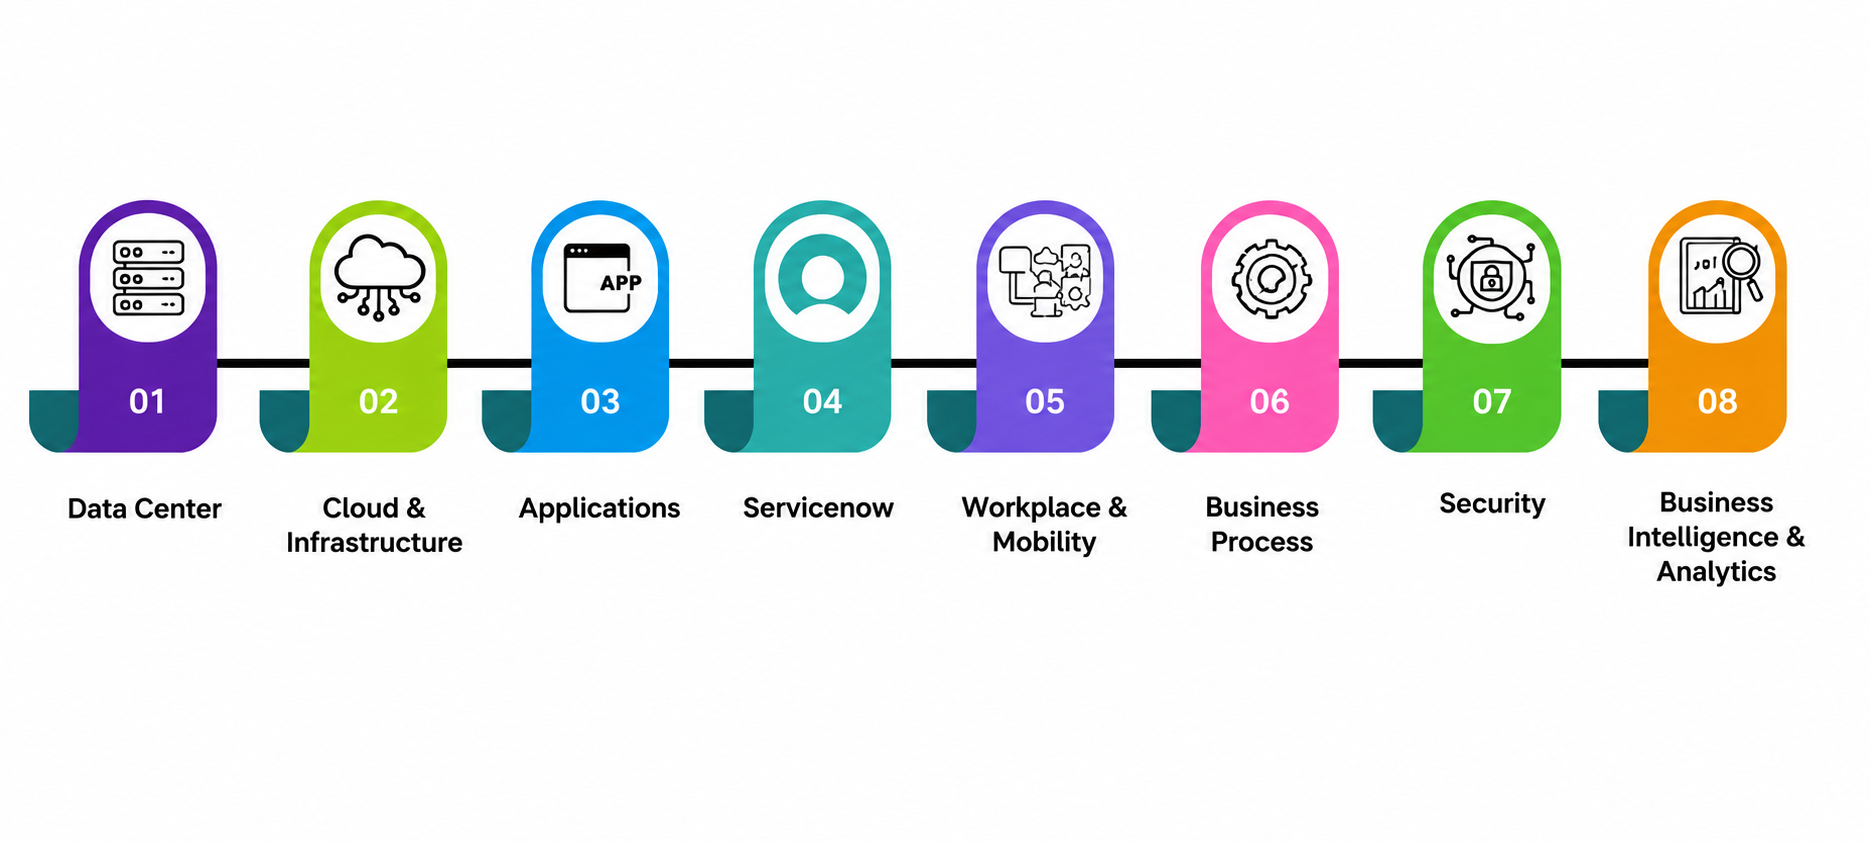
\includegraphics[width=0.95\textwidth]{services_diagram.png}
    \caption{Main business areas and services of DXC Technology Morocco}
    \label{fig:services-diagram}
\end{figure}

\subsubsection{Organizational Structure}

DXC Technology Morocco is organized into different functional and operational
structures that support the delivery of technology services to its customers.
These structures include management and support functions as well as specialized
service lines responsible for delivering technical and business solutions.

Figure~\ref{fig:dxc-org} presents an overview of the organizational structure
of DXC Technology Morocco.

\begin{figure}[H]
    \centering
    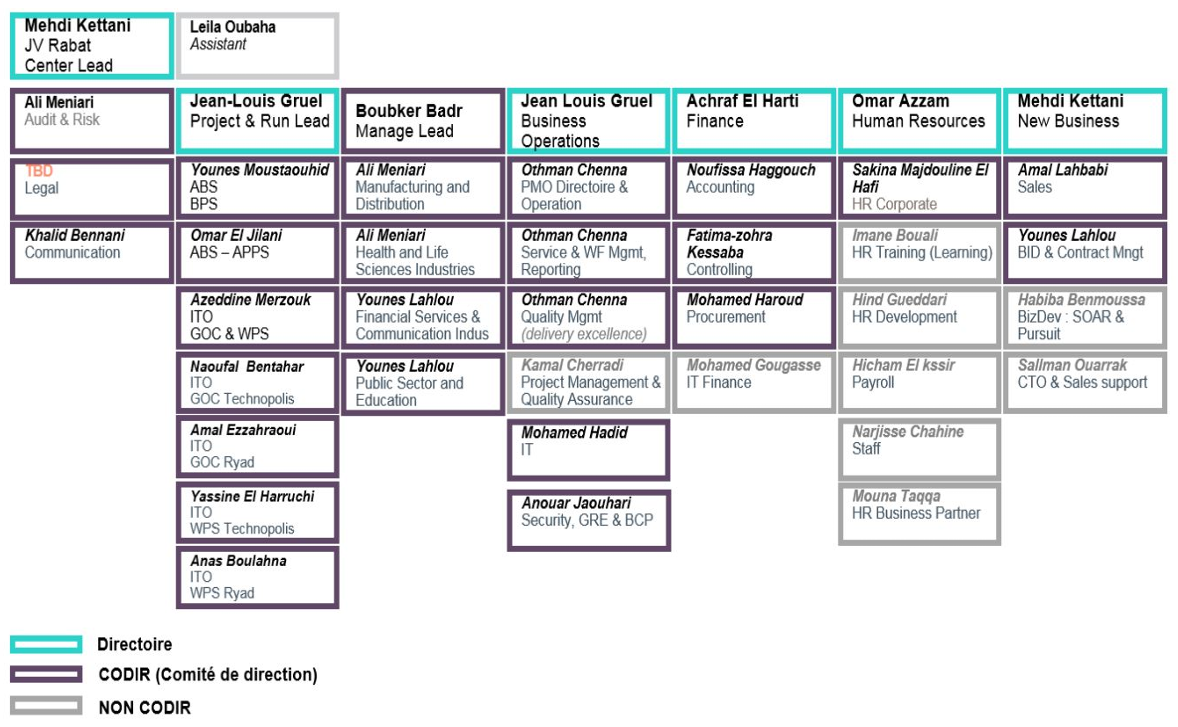
\includegraphics[width=0.95\textwidth]{dxc_org.png}
    \caption{Organizational structure of DXC Technology Morocco}
    \label{fig:dxc-org}
\end{figure}


\subsubsection{Clients and Strategic Partners}

DXC Technology Morocco serves organizations operating across a wide range of
industries, including manufacturing, retail, banking and finance,
telecommunications, energy, healthcare, transportation, tourism, the public
sector, and real estate.

The diversity of its customer base reflects the broad range of technology and
business services provided by the organization.

\begin{figure}[H]
    \centering
    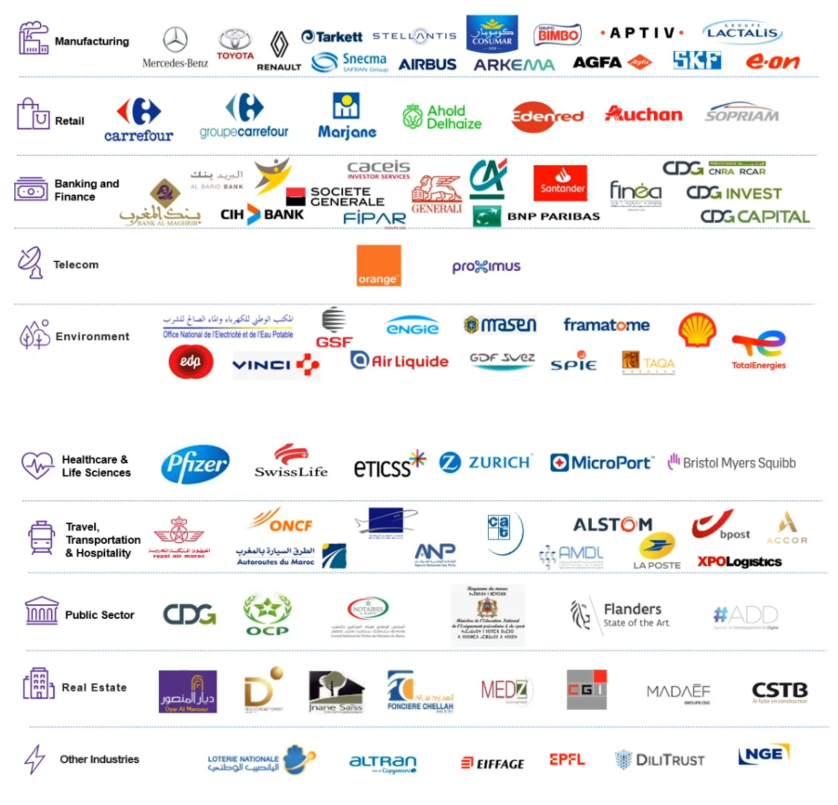
\includegraphics[width=0.9\textwidth]{dxc_clients.png}
    \caption{Examples of DXC Technology Morocco's clients}
    \label{fig:dxc-clients}
\end{figure}

DXC Technology Morocco also works with technology partners and maintains
industry certifications that support the quality, security, and reliability
of its services. These partnerships and certifications contribute to the
company's ability to deliver solutions that meet technological and operational
requirements.

\begin{figure}[H]
    \centering
    
\includegraphics[width=0.75\textwidth]{dxc_partners_certifications.png}
    \caption{Selected partners and certifications of DXC Technology Morocco}
    \label{fig:dxc-partners}
\end{figure}

\section{Internship Context}

\subsection{Internship Framework}

As part of my academic curriculum, I completed a two-month PFA internship at
\textbf{DXC Technology Morocco}. The internship was conducted entirely remotely
and focused on the discovery and practical application of the ServiceNow
platform.

The internship was supervised by \textbf{Houda AJDIR}, who provided guidance,
clarifications, and feedback throughout the internship. The work was carried
out independently, with regular communication with the company supervisor
regarding the progress and requirements of the assigned work.

\subsection{Internship Objectives}

The main objective of this internship was to develop practical knowledge of the
\textbf{ServiceNow} platform and gain experience in its administration and
configuration within a professional IT environment.

More specifically, the internship aimed to:

\begin{itemize}
    \item Acquire a solid understanding of the ServiceNow platform and its
    main administration concepts through the System Administrator training.

    \item Develop an understanding of \textbf{IT Service Management (ITSM)}
    concepts and their implementation within ServiceNow.

    \item Apply the knowledge acquired during the training to a practical
    ServiceNow project.

    \item Design and configure a structured \textbf{Service Request Fulfillment}
    solution for managing IT service requests.

    \item Gain practical experience with ServiceNow configuration components,
    including forms, workflows, approval processes, assignment rules,
    notifications, and business rules.

    \item Understand how automation can be used to improve the processing,
    traceability, and fulfillment of IT service requests.

    \item Develop the ability to work independently, organize tasks
    effectively, and manage a technical project in a remote working
    environment.
\end{itemize}

\subsection{Remote Working Environment}

The internship was conducted entirely remotely, without any physical presence
at the company's premises. This working arrangement required me to organize my
work independently and manage my time according to the objectives and
requirements of the internship.

Throughout the internship, the main channel of communication was with my
company supervisor, \textbf{Houda AJDIR}. She provided the necessary guidance,
clarifications, and feedback regarding the training and the assigned project.

The remote nature of the internship also required a high degree of autonomy
and personal organization. Tasks were carried out independently, while
progress and questions were communicated to the supervisor when necessary.
This environment allowed me to develop my ability to manage my workload,
solve problems independently, and maintain progress throughout the different
stages of the internship.

\subsection{Internship Phases}

The internship was organized into two main phases, each with a specific
objective. The first phase focused on acquiring the necessary knowledge of
the ServiceNow platform, while the second phase consisted of applying this
knowledge to a practical project.

\begin{table}[H]
    \centering
    \begin{tabular}{|c|c|p{8cm}|}
        \hline
        \textbf{Phase} & \textbf{Duration} & \textbf{Main Activities} \\ \hline
        
        Phase 1 & First Month &
        ServiceNow System Administrator training, covering the fundamental
        concepts of the platform and its administration and configuration. \\ \hline
        
        Phase 2 & Second Month &
        Design and implementation of the Service Request Fulfillment project,
        including the configuration and testing of the required ServiceNow
        components. \\ \hline
    \end{tabular}
    \caption{Organization of the Internship}
    \label{tab:internship-phases}
\end{table}

During the first phase, the focus was on building a solid foundation in
ServiceNow administration. The training provided the knowledge required to
understand the platform and its main configuration concepts.

During the second phase, the knowledge acquired during the training was applied
to the development of the Service Request Fulfillment solution. This phase
involved analyzing the requirements, designing the service processes,
configuring the ServiceNow components, and testing the resulting solution.


\section{Project Context}

\subsection{Background (Service Request Management)}
In modern enterprise environments, Information Technology Service Management (ITSM) is critical 
for aligning  IT services with business needs. Within the ITSM framework, Request Fulfillment is 
the core process responsible for managing the lifecycle of all standard service requests from users. 
These requests typically include access to applications, software installations, hardware provisioning, 
and routine information queries. An effective Request Fulfillment process ensures that employees 
have access to the IT resources they need to perform their daily tasks efficiently, while the 
organization maintains proper authorization, compliance, and security controls.

\subsection{Problem Statement}
Despite the critical nature of IT services, many organizations continue to rely
on manual or fragmented processes to handle user requests. When requests are
submitted via unstructured channels such as emails, phone calls, or direct
messages, several operational issues arise:

\begin{itemize}

    \item \textbf{Lack of Traceability:} It is difficult to track the status of
    a request, leading to poor visibility for both the end-user and the IT
    support team.

    \item \textbf{Delayed Processing:} Manual routing of requests for
    managerial or security approvals often creates bottlenecks, increasing
    the time required to fulfill the request.

    \item \textbf{Assignment Errors:} Without an automated routing mechanism,
    requests are frequently assigned to the wrong fulfillment group, causing
    further delays.

    \item \textbf{Absence of Metrics:} The inability to track request
    fulfillment times makes it difficult to measure performance against
    Service Level Agreements (SLAs) or identify areas for continuous
    improvement.

\end{itemize}

These challenges highlight the need for a structured and automated request
fulfillment process that ensures requests are properly captured, authorized,
assigned, and monitored throughout their lifecycle.

\subsection{Project Objectives}
To address these operational inefficiencies, this project aims to design and implement an automated 
Request Fulfillment solution using the ServiceNow platform. The primary objectives are : 
\begin{itemize}
\item \textbf{Centralize Requests:} Provide a single, structured portal (Service Catalog) 
where users can easily and intuitively submit IT requests.
\item \textbf{Automate Workflows:} Replace manual approval and routing steps with automated 
workflows to ensure requests are immediately directed to 
the appropriate managers and fulfillment teams.
\item \textbf{Standardize Data Collection:} Use dynamic request forms to ensure all 
necessary information is captured at the time of submission, 
eliminating back-and-forth communication.
\item \textbf{Enforce SLAs:} Configure Service Level Agreements to monitor
fulfillment times and trigger automated escalations when targets are at risk.
\item \textbf{Improve Traceability:} Provide visibility into the status and
progress of requests throughout their fulfillment lifecycle.
\end{itemize}

\subsection{Project Scope}
The scope of this project encompasses the end-to-end configuration of five specific Service 
Catalog items that represent common and critical IT request : 
% return for this to check if there is some shit you didn't really fucking do
\begin{enumerate}
    \item \textbf{User Account Creation:} Automating the approval and task generation for 
    provisioning Active Directory, email, and application accounts for new employees.
    \item \textbf{Enterprise VPN Access:} Structuring the security and network 
    approval chains required for secure remote access.
    \item \textbf{Software Installation:} Managing software requests including automated 
    license verification and installation tasks.
    \item \textbf{IT Hardware Requests:} Automating the process from stock verification and 
    procurement approval to delivery and configuration.
    \item \textbf{Password Reset:} Implementing a secure, streamlined process for routine 
    account recovery.
\end{enumerate}
The technical scope involves leveraging ServiceNow's core capabilities, including the Service 
Catalog, Flow Designer for process automation, Business Rules and Client Scripts for backend 
logic, with UI Policies, User Criteria for access control, and SLA definitions.

\subsection{Project Deliverables}
The main deliverable of the project was a configured ServiceNow Request
Fulfillment solution covering five IT service catalog items. The solution
included structured request forms, approval and fulfillment processes,
assignment mechanisms, notifications, and Service Level Agreements.

The project also resulted in configuration artifacts that could be packaged
using ServiceNow Update Sets to support the controlled migration of the
developed solution between environments.


\section{Methodological Approach}
To ensure the successful delivery of the Request Fulfillment solution, a structured and iterative 
methodological approach was adopted. The project was executed through the following key phases: 
\begin{itemize}
\item \textbf{Requirements Analysis:} Defining the specific inputs, 
variables, approval chains, and fulfillment tasks required for each 
of the five catalog items. This phase involved translating 
business requirements into technical ServiceNow specifications.
\item \textbf{Platform Configuration and Development:} Utilizing a ServiceNow Development 
instance to build the solution. This involved creating Catalog Items, defining variables and 
UI Policies for dynamic forms, and utilizing Flow Designer to build the underlying 
automation logic.
\item \textbf{Testing and Validation:} Conducting rigorous testing of each workflow to ensure 
approvals trigger correctly, tasks are assigned to the right fulfillment groups based on the 
request type, and SLAs attach properly based on ticket priority.
\item \textbf{Deployment Preparation:} Packaging the configurations into ServiceNow Update 
Sets to ensure a safe, structured, and traceable migration of the developed features from 
the Development environment to Testing (UAT) and Production environments.
\end{itemize}

\begin{figure}[H]
    \centering
    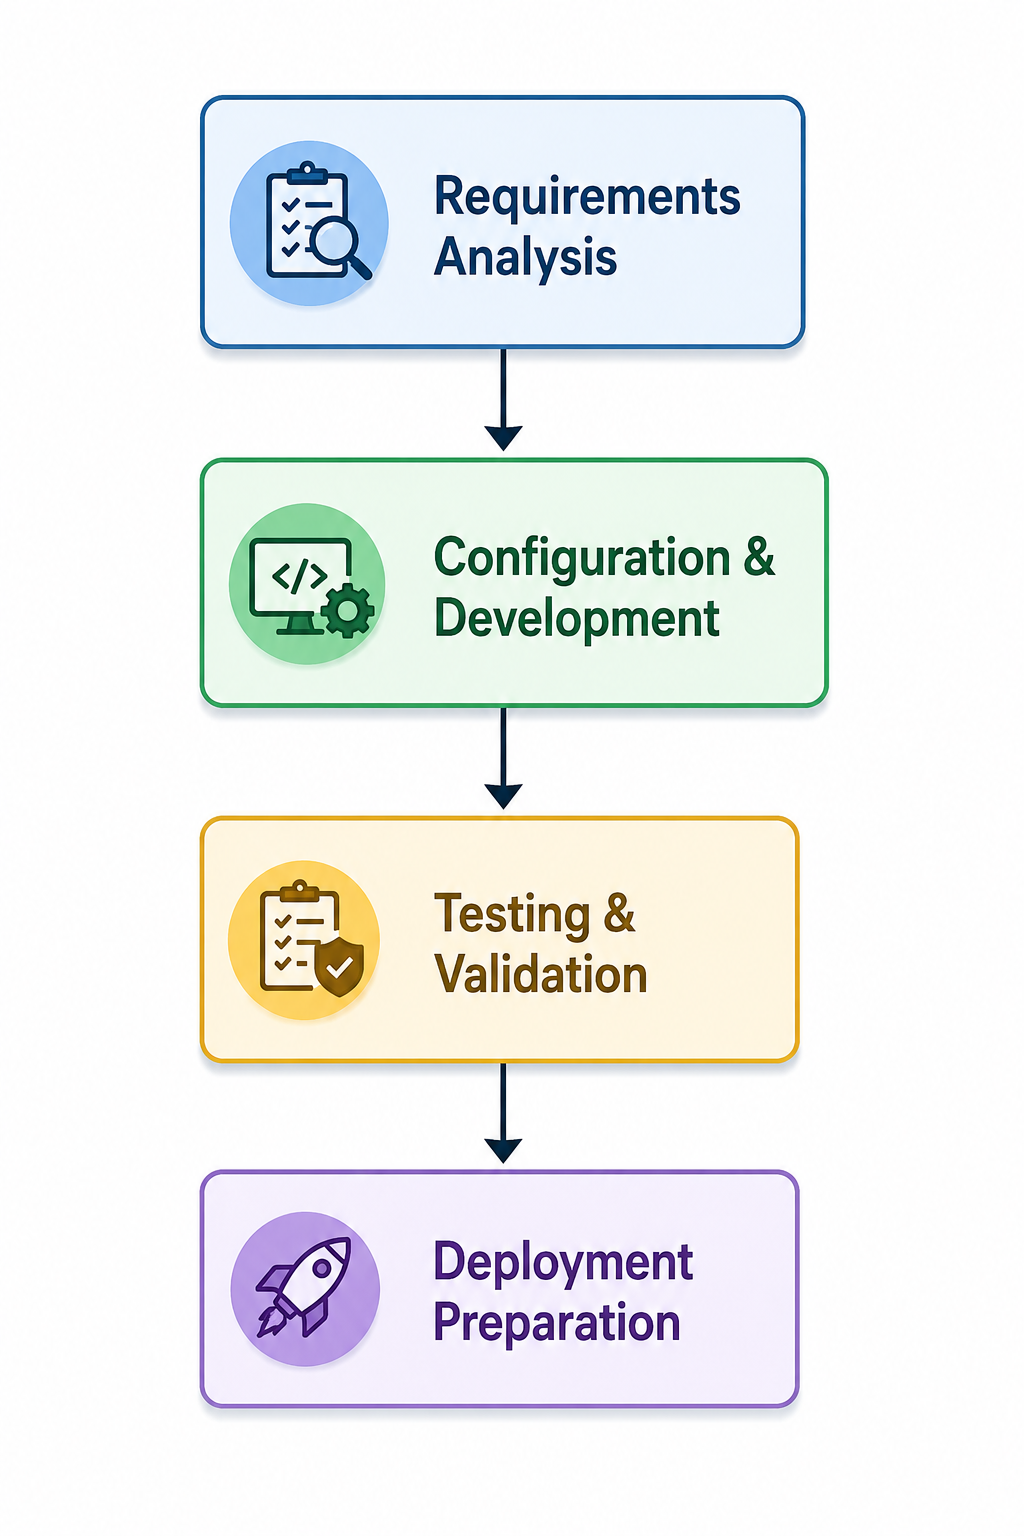
\includegraphics[width=0.35\textwidth]{methodological_approach.png}
    \caption{Methodological Approach Phases}
    \label{fig:methodological_approach}
\end{figure}

\section{Conclusion}
This chapter presented the context of the internship at DXC Technology Morocco,
the Service Request Fulfillment project, its objectives and scope, and the
methodological approach adopted. The following chapter introduces the ServiceNow
platform, IT Service Management (ITSM), and the main technical concepts used in
the project.


\chapter{Theoretical and Technical Background}

\section{Introduction}
This chapter presents the theoretical and technical concepts required to understand the 
Service Request Fulfillment solution developed during the internship. It introduces the 
ServiceNow platform, its architecture, and its core capabilities. Furthermore, it explores 
the principles of Information Technology Service Management (ITSM) and the role of ITIL best 
practices in service request management. Finally, the chapter details the main ServiceNow 
components used to design, automate, and prepare the deployment of the solution, 
including the Service Catalog, Flow Designer, Service Level Agreements (SLAs), and the 
ServiceNow development lifecycle.

\section{ServiceNow Platform}

\begin{figure}[H]
    \centering
    
\includegraphics[width=0.35\textwidth]{ServiceNow_logo.png}
    \caption{ServiceNow Logo}
    \label{fig:serviceNow_logo}
\end{figure}

\subsection{Overview of ServiceNow}
ServiceNow is a cloud-based enterprise platform that provides Software as a
Service (SaaS) and Application Platform as a Service (aPaaS) solutions. It is
designed to support the management and automation of enterprise processes and
services. Initially focused on Information Technology Service Management (ITSM),
the platform has progressively expanded its capabilities to cover different
areas of an organization, including IT operations, security, human resources,
customer service, and business processes.

The platform provides a centralized environment in which organizations can
define processes, manage requests, automate tasks, and monitor their execution.
Its configurable architecture also allows organizations to adapt the platform
to their specific business and operational requirements.


\begin{table}[H]
    \centering
    \begin{tabular}{|l|l|}
        \hline
        \textbf{Founded} & 2004 \\ \hline
        \textbf{Founded by} & Fred Luddy \\ \hline
        \textbf{Headquarters} & Santa Clara, California, USA \\ \hline
        \textbf{Logo} & \includegraphics[width=0.2\textwidth]{serviceNow_logo.png} \\ \hline
        \textbf{Website} & \href{https://www.servicenow.com/}{Servicenow.com} \\ \hline
    \end{tabular}
    \caption{ServiceNow Overview}
    \label{tab:servicenow-overview}
\end{table}

\subsection{ServiceNow Architecture}
ServiceNow is based on a cloud architecture designed to provide each customer with and isolated 
and configurable environment. One of the main characteristics of the platform is its 
\textbf{multi-instance architecture}, in which each customer is provided with a dedicated instance.

Unlike a traditional multi-tenant architecture, where multiple customers share the same application 
environment, the multi-instance approach provides a greater level of isolation between customer environments. 
Each instance contains its own application, middleware, and database resources, while the underlying 
physical infrastructure can be shared.

\begin{figure}[H]
    \centering
    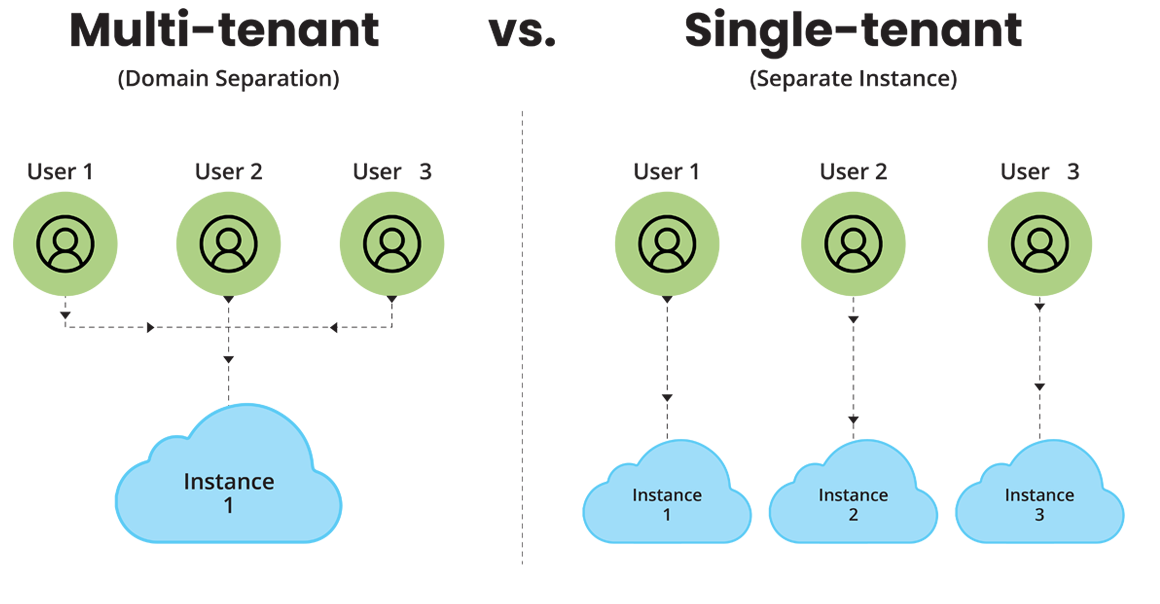
\includegraphics[width=0.85\textwidth]{Servicenow-domain-separation-multi-tenant.png}
    \caption{Multi Tenant vs Single Tenant}
    \label{fig:Servicenow-domain-separation-multi-tenant}
\end{figure}

This architecture provides several advantages, particularly in terms of data isolation, configuration 
flexibility, and platform management. changes or configurations made within one instance are isolated 
from other customer instances, allowing organizations to adapt the platform to their specific requirements.

\begin{figure}[H]
    \centering
    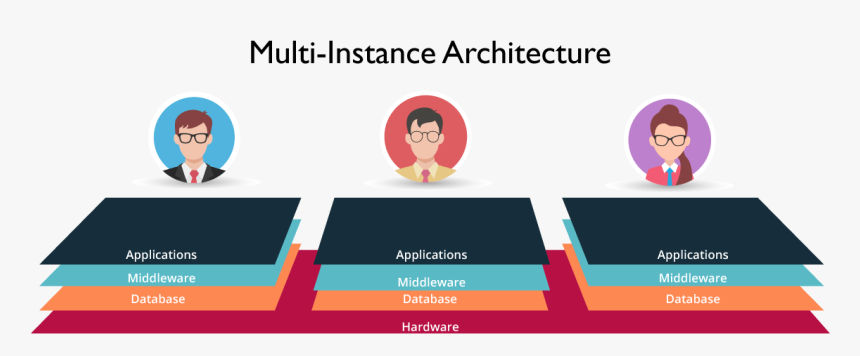
\includegraphics[width=0.85\textwidth]{servicenow_multi_instance.png}
    \caption{Multi-Instance Architecture of ServiceNow}
    \label{fig:servicenow-multi-instance}
\end{figure}

\subsection{ServiceNow Applications and Modules}
ServiceNow provides a wide range of applications and modules designed to support different organizational 
processes and address specific enterprise needs :

\begin{itemize}
    \item \textbf{ITSM (IT Service Management):} The core module focused on delivering and managing IT services, encompassing incident, 
    problem, change, and request management.
    \item \textbf{ITOM (IT Operations Management):} Focuses on infrastructure visibility, service health, and cloud provisioning.
    \item \textbf{ITBM (IT Business Management):} Aligns IT investments with business goals through project portfolio management and 
    financial tracking.
    \item \textbf{Security Operations:} Integrates security incident response and vulnerability management directly into IT workflow.
\end{itemize}

This project is built primarily on the ITSM module, leveraging its Service Catalog and workflow automation capabilities.

\subsection{ServiceNow Development and Configuration}
ServiceNow is a low-code/no-code platform that allows organizations to build
and customize applications rapidly. Many processes can be configured using
graphical interfaces and predefined platform components, reducing the need
for extensive programming. However, the platform also provides scripting
capabilities for implementing more complex business logic and extending
standard functionality.

JavaScript is the primary scripting language used within ServiceNow. It can
be used to implement server-side logic, control client-side behavior, validate
data, and automate specific operations according to business requirements.
This combination of configuration and scripting allows developers to adapt the
platform while maintaining a flexible and scalable development environment.

For the Service Request Fulfillment project, ServiceNow configuration was
mainly used to create and customize Service Catalog items, define request
variables, control form behavior, configure approval and fulfillment
processes, establish assignment rules and notifications, and implement
Service Level Agreements (SLAs). These elements provided the technical
foundation for the automation of the request fulfillment processes.

\section{Information Technology Service Management (ITSM)}

\subsection{ITSM Overview}
Information Technology Service Management (ITSM) is a strategic approach to
designing, delivering, managing, and improving the way information technology
services are provided within an organization. The primary objective of ITSM is
to ensure that the appropriate processes, people, and technologies are in
place to support the organization in achieving its business goals. This
approach shifts the focus from managing isolated IT infrastructure components
to delivering integrated and effective IT services.

\subsection{ITIL and Service Management}
ITIL(Information Technology Infrastructure Library) is a widely adopted framework that provides 
guidance and best practices fir IT Service Management. It helps organizations establish structured 
approaches for designing, delivering, supporting, and continually improving IT-enabled services. 

ITIL emphasizes the importance of defining clear processes, responsibilities, and service objectives. 
Its practices can be adapted to the specific requirements of an organization rather than being implemented as a 
rigid set of procedures.

For this project, ITIL concepts provide a general framework for understanding
service request management and the importance of standardized processes,
defined approval procedures, controlled fulfillment, and service-level
monitoring.

\subsection{Service Request Management}
Service Request Management is an ITSM practice focused on handling standard
requests submitted by users for predefined IT services. These requests may
include application access, software installation, hardware requests, or
password resets.

A structured request management process ensures that requests are properly
recorded, validated, authorized, assigned, fulfilled, and closed. This
improves the consistency and traceability of service delivery while ensuring
that requests follow predefined procedures.

In ServiceNow, Service Request Management is supported by the
\textbf{Service Catalog}, which provides users with a structured interface
for submitting requests. Each catalog item defines the required information
and can be associated with approval processes, fulfillment tasks, assignment
rules, notifications, and automation.

The process can therefore be summarized through several main activities:
request submission, approval, assignment, fulfillment, and closure. In the
context of this project, five types of IT service requests were considered:

\begin{enumerate}
    \item \textbf{User Account Creation}
    \item \textbf{Enterprise VPN Access}
    \item \textbf{Software Installation}
    \item \textbf{IT Hardware Requests}
    \item \textbf{Password Reset}
\end{enumerate}

These request types form the basis of the Service Request Fulfillment
solution developed during the internship.

\subsection{Request Fulfillment Lifecycle}
The fulfillment of an IT service request follows a structured lifecycle that
ensures the request is properly processed from submission to completion. A
typical request fulfillment process consists of several stages, including
submission, approval, assignment, fulfillment, and closure.

\begin{enumerate}
    \item \textbf{Request Submission:} The user selects the required service
    and provides the necessary information through the Service Catalog.

    \item \textbf{Approval:} The request is reviewed and, when required,
    submitted to the appropriate person or department for approval.

    \item \textbf{Assignment:} Once approved, the request is assigned to the
    appropriate fulfillment group or generates the required fulfillment tasks.

    \item \textbf{Fulfillment:} The responsible team performs the activities
    required to provide the requested service.

    \item \textbf{Closure:} After the required activities are completed, the
    request is validated and closed.
\end{enumerate}

In ServiceNow, these stages can be supported and automated through workflows,
approvals, task assignment, notifications, and other platform capabilities.
This automation helps reduce manual processing, improve traceability, and
ensure that requests follow a consistent fulfillment process.

Figure~\ref{fig:request-fulfillment-lifecycle} illustrates the main stages of
the request fulfillment lifecycle.

\begin{figure}[H]
    \centering
    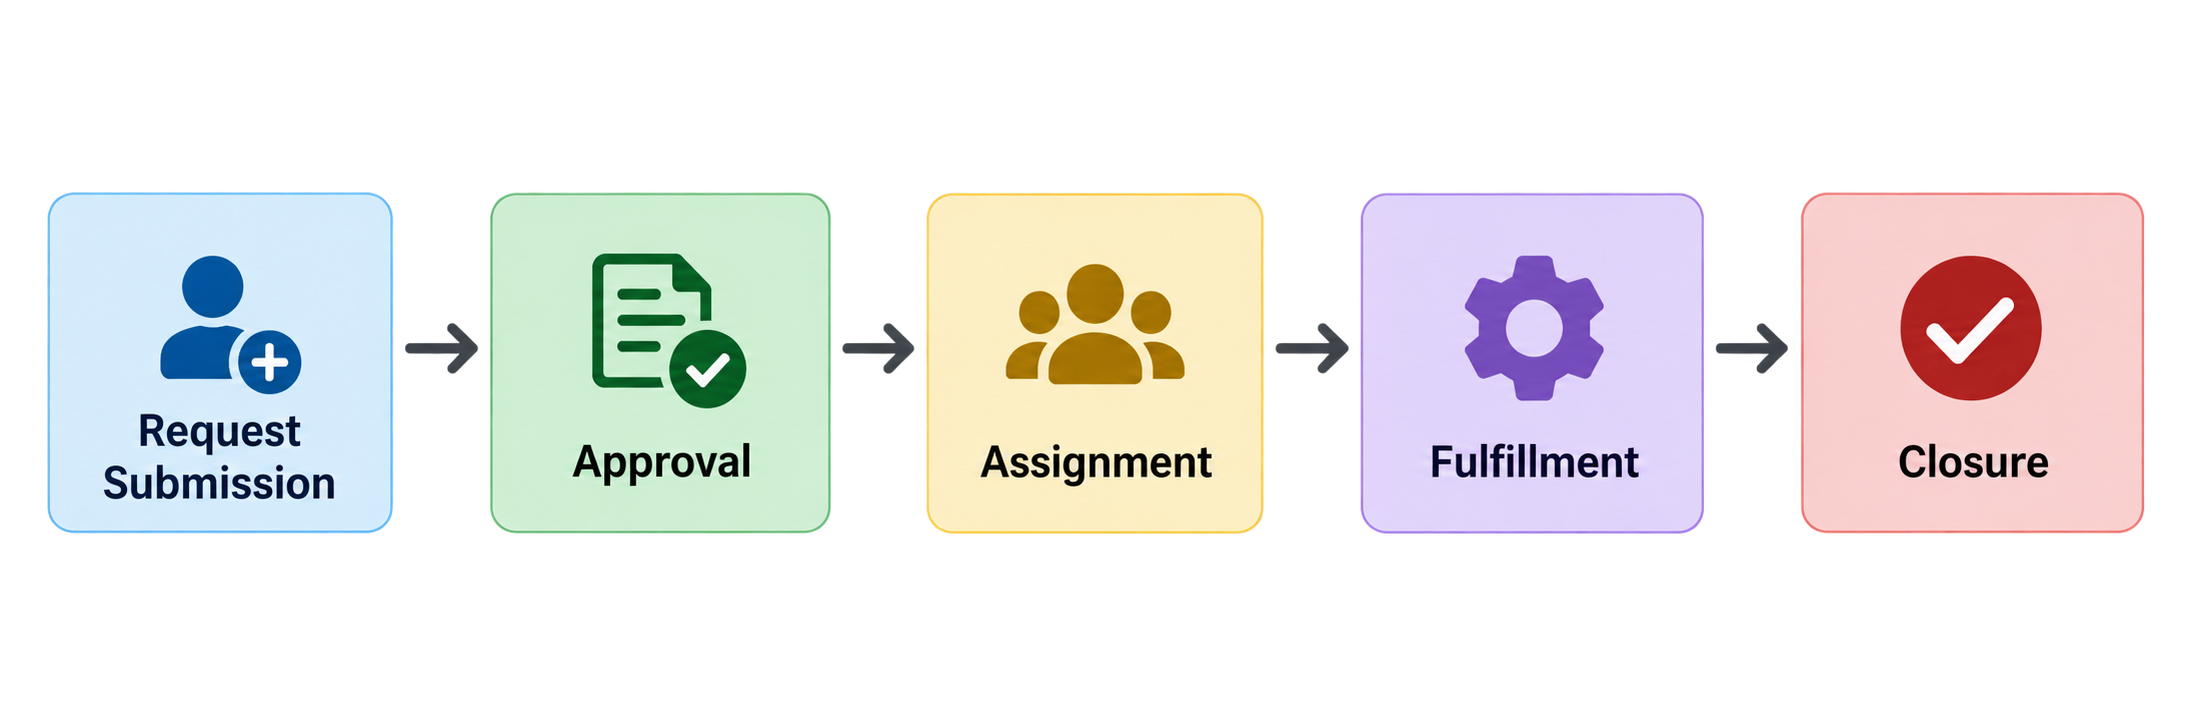
\includegraphics[width=0.9\textwidth]{request-fulfillment-lifecycle.png}
    \caption{Request Fulfillment Lifecycle in ServiceNow}
    \label{fig:request-fulfillment-lifecycle}
\end{figure}

\section{ServiceNow Service Catalog}

\subsection{Service Catalog and Catalog Items}
The Service Catalog is the user-facing interface of the ITSM module, providing
a centralized portal where employees can browse, search for, and request
predefined IT services. It standardizes the submission of service requests by
providing structured forms and ensuring that the necessary information is
collected from the beginning of the request process.

Catalog Items represent the individual services available for request within
the Service Catalog. Each item is designed to address a specific user need
and can be organized into appropriate categories to facilitate navigation and
selection.

For this project, five Catalog Items were designed to address common IT
service needs: \textbf{User Account Creation}, \textbf{Enterprise VPN Access},
\textbf{Software Installation}, \textbf{IT Hardware Requests}, and
\textbf{Password Reset}. Each item was configured with the information and
process requirements necessary for its subsequent fulfillment.

\subsection{Catalog Configuration and Access Control}
ServiceNow provides several configuration features that allow Catalog Items to
be adapted to the specific requirements of each service. One of the main
elements is the use of \textbf{variables}, which define the information that
users must provide when submitting a request. Variables can be used to
collect different types of information, such as text, selections, dates, or
references to existing records.

\textbf{Variable Sets} can also be used to group related variables and reuse
them across multiple Catalog Items. This helps maintain consistency and
reduces the need to configure the same information repeatedly.

The behavior and visibility of form fields can be controlled using
\textbf{UI Policies}. These policies allow fields to be made mandatory,
visible, or read-only depending on the conditions defined for a request.
This makes it possible to create dynamic forms that display only the
information relevant to the selected service.

Access to Catalog Items can be managed using \textbf{User Criteria}, which
define which users or groups are authorized to access specific services.
This ensures that catalog services are presented only to the appropriate
users according to the organization's access requirements.

For the Service Request Fulfillment project, these configuration mechanisms
were used to structure the request forms, collect the required information,
control form behavior, and manage access to the different Catalog Items.

\subsection{Catalog Configuration and Access Control}

To collect the information required for a specific request, Catalog Items use
\textbf{Variables} and \textbf{Variable Sets}, which act as input fields on
the request form. These elements allow each Catalog Item to collect the
information needed for its specific fulfillment process.

To provide a consistent user experience, \textbf{UI Policies} and
\textbf{Client Scripts} can be used to dynamically control form fields,
making them visible, mandatory, or read-only according to predefined
conditions. In addition, \textbf{User Criteria} can be used to control access
to Catalog Items and ensure that services are available only to authorized
users.

For the Service Request Fulfillment project, these configuration features
were used to structure the request forms, collect the required information,
control form behavior, and manage access to the different services.


\section{Workflow Automation}

\subsection{Flow Designer and Process Automation}

\textbf{Flow Designer} is ServiceNow's visual automation tool for creating
multi-step processes. It allows developers to define a sequence of actions
that are automatically executed when a predefined trigger occurs. These
actions can include creating tasks, requesting approvals, updating records,
and sending notifications.

Flow Designer helps replace manual routing and processing by connecting the
different stages of a service request into a structured workflow. In the
Service Request Fulfillment project, it was used to automate the processing
of requests and coordinate their approval and fulfillment activities.

ServiceNow also supports backend automation through \textbf{Business Rules}.
These server-side scripts execute when records are inserted, updated, or
queried, allowing additional business logic to be applied to the system.
Together, Flow Designer and Business Rules provide mechanisms for automating
both process-level and record-level operations.

\subsection{Approvals, Tasks, and Notifications}

Automated workflows rely on approvals, fulfillment tasks, and notifications
to coordinate the different stages of a request.

\begin{itemize}
    \item \textbf{Approvals:} Approval requests are generated when a service
    requires authorization before fulfillment can continue. The approval
    process can involve managers or other responsible teams depending on the
    type of request.

    \item \textbf{Catalog Tasks (SCTASKs):} Once the required approvals are
    completed, fulfillment tasks can be generated and assigned to the
    appropriate support groups. These tasks represent the activities required
    to complete the requested service.

    \item \textbf{Notifications:} Automated notifications keep users and
    stakeholders informed about important events, such as pending approvals,
    task assignments, status changes, and request completion.
\end{itemize}

These mechanisms work together to provide a structured and traceable
fulfillment process.


\section{Service Level Agreements}

\subsection{SLA Concepts}

A \textbf{Service Level Agreement (SLA)} is a documented commitment that
defines the expected level of service and measurable performance targets.
SLAs commonly specify response or fulfillment times and provide a basis for
monitoring service performance.

In IT Service Management, SLAs help establish clear expectations, measure
performance, and identify requests that are approaching or exceeding their
defined service targets.

\subsection{SLA Management in ServiceNow}

In ServiceNow, \textbf{SLA Definitions} establish the conditions used to
track the time associated with a record. These definitions can specify when
an SLA starts, pauses, resumes, and stops according to predefined conditions.

ServiceNow continuously tracks active SLAs and provides visibility into the
remaining time and current status of each target. This allows support teams
to monitor fulfillment performance and identify requests that may require
attention before an SLA is breached.

For the Service Request Fulfillment project, SLAs were considered to monitor
the time required to process service requests and to support compliance with
defined fulfillment targets.


\section{Development and Deployment}

\subsection{Development and Testing Environments}

ServiceNow development commonly uses separate environments for development,
testing, and production. This separation allows configurations to be
developed and validated before they are made available to end users.

The main environments used in a typical ServiceNow development lifecycle are:

\begin{itemize}
    \item \textbf{DEV:} The development environment where configurations,
    Catalog Items, forms, and workflows are created and modified.

    \item \textbf{TEST (UAT):} The testing environment used to validate the
    developed solution and verify that it meets the defined requirements.

    \item \textbf{PROD:} The production environment where the validated
    solution is made available to end users.
\end{itemize}

This separation contributes to a controlled development process and reduces
the risk of introducing untested changes into the production environment.

\subsection{Update Sets and Deployment}

An \textbf{Update Set} is a ServiceNow mechanism used to capture and organize
configuration changes made within an instance. It allows related
customizations to be packaged and transferred between ServiceNow
environments.

Update Sets can contain different configuration elements, such as Catalog
Items, workflows, business rules, client scripts, and UI policies. They
therefore facilitate the controlled migration of developed configurations
from a development environment to a testing or production environment.

For this project, Update Sets were used to organize the developed
configurations and prepare them for controlled migration between the
different ServiceNow environments.


\section{Conclusion}

This chapter presented the main theoretical and technical concepts underlying
the Service Request Fulfillment project. It introduced ServiceNow, ITSM,
Service Request Management, the Service Catalog, workflow automation, SLAs,
and the development and deployment process. These concepts provide the
foundation for the following chapters, which focus on the design and practical
implementation of the developed solution.

\chapter{Analysis and Design of the Service Request Fulfillment Solution}

\section{Introduction}
This chapter bridges the gap between the theoretical concepts of ITSM and the
practical design of the Service Request Fulfillment solution. It provides an
analysis of the existing request management process, identifying its current
limitations and defining the functional requirements for the proposed
solution. The chapter then presents the solution design, including the
proposed ServiceNow architecture, the structure of the Service Catalog, and
the data model. Finally, it provides a detailed design specification for each
of the five core Catalog Items, including their respective inputs, approval
workflows, and Service Level Agreements (SLAs).

\section{Analysis of the Existing Request Management Process}
\subsection{Existing Process and Current Challenges}
Prior to the implementation of the proposed solution, IT service requests were managed through 
different communication channels, requiring IT support personnel to manually review, process, and route each request. 
This approach presented several operational challenges : 

\begin{itemize}
    \item \textbf{Data Inconsistency:} Without standardized request forms,
    submitted requests may lack important information required for their
    processing and fulfillment, resulting in additional communication with
    the requester.

    \item \textbf{Manual Routing and Approval:} Requests and approval steps
    may require manual intervention to identify the appropriate responsible
    person or fulfillment group, which can increase processing time.

    \item \textbf{Lack of Visibility:} Without a centralized system for
    managing requests, users and support teams have limited visibility into
    the status and progress of ongoing requests.

    \item \textbf{Limited Performance Monitoring:} The absence of centralized
    request tracking makes it difficult to consistently monitor fulfillment
    times, evaluate service performance, and identify process bottlenecks.
\end{itemize}

These limitations highlighted the need for a centralized and automated
solution capable of standardizing request submission, automating approval and
routing processes, and improving the overall traceability of IT service
requests.

\subsection{Requirements Analysis}
Based on the analysis of the existing request management process, a set of
functional requirements was defined for the proposed Service Request
Fulfillment solution. These requirements describe the main capabilities that
the system should provide to standardize and automate the handling of IT
service requests.

The solution should meet the following functional requirements:
\begin{itemize}
    \item \textbf{Request Submission:} Provide users with a centralized
    Service Catalog through which they can select and submit predefined IT
    service requests.

    \item \textbf{Structured Data Collection:} Provide dedicated request
    forms containing the information required for each type of service.

    \item \textbf{Approval Management:} Support predefined approval processes
    for requests that require authorization before fulfillment.

    \item \textbf{Automatic Assignment:} Route requests and fulfillment tasks
    to the appropriate support groups according to predefined rules.

    \item \textbf{Workflow Automation:} Automate the different stages of the
    request fulfillment process, from submission and approval to task
    completion and closure.

    \item \textbf{Notifications:} Inform users and relevant stakeholders
    about important events and changes in the request lifecycle.

    \item \textbf{SLA Management:} Support the monitoring of fulfillment
    times according to predefined service-level targets.

    \item \textbf{Request Tracking:} Provide centralized visibility into the
    status and progress of submitted requests.

\end{itemize}

These requirements served as the basis for designing the proposed ServiceNow
solution and defining the configuration of the different Catalog Items and
fulfillment workflows.

\section{Functional Analysis}

\subsection{Actors and Responsibilities}
The Service Request Fulfillment process involves several actors who interact with the system 
at different stages of the request lifecycle. Each actor has specific responsibilities related 
to the submission, authorization, and fulfillment of service requests. 

The main actors identified for the proposed solution are : 

\begin{itemize}
    \item \textbf{Requester:} The employee who submits an IT service request
    through the Service Catalog and provides the information required for its
    processing.

    \item \textbf{Direct Manager:} The responsible person who reviews and approves
    requests when managerial authorization is required.

    \item \textbf{Fulfillment Teams:} The teams responsible for
    processing assigned fulfillment tasks and providing the requested service.

    \item \textbf{HR Team:} The responsible team involved in requests that
    require employee-related validation, such as account creation.

    \item \textbf{Security Team:} The team responsible for
    reviewing and processing requests related to secure access and network
    services, such as Enterprise VPN Access.
\end{itemize}

The interaction between these actors depends on the type of service
requested. A request may therefore involve one or more approval and
fulfillment stages before it can be completed.

Figure~\ref{fig:use-case-diagram} illustrates the main actors involved in the
Service Request Fulfillment process and their interactions with the proposed
solution.


\begin{figure}[H]
    \centering
    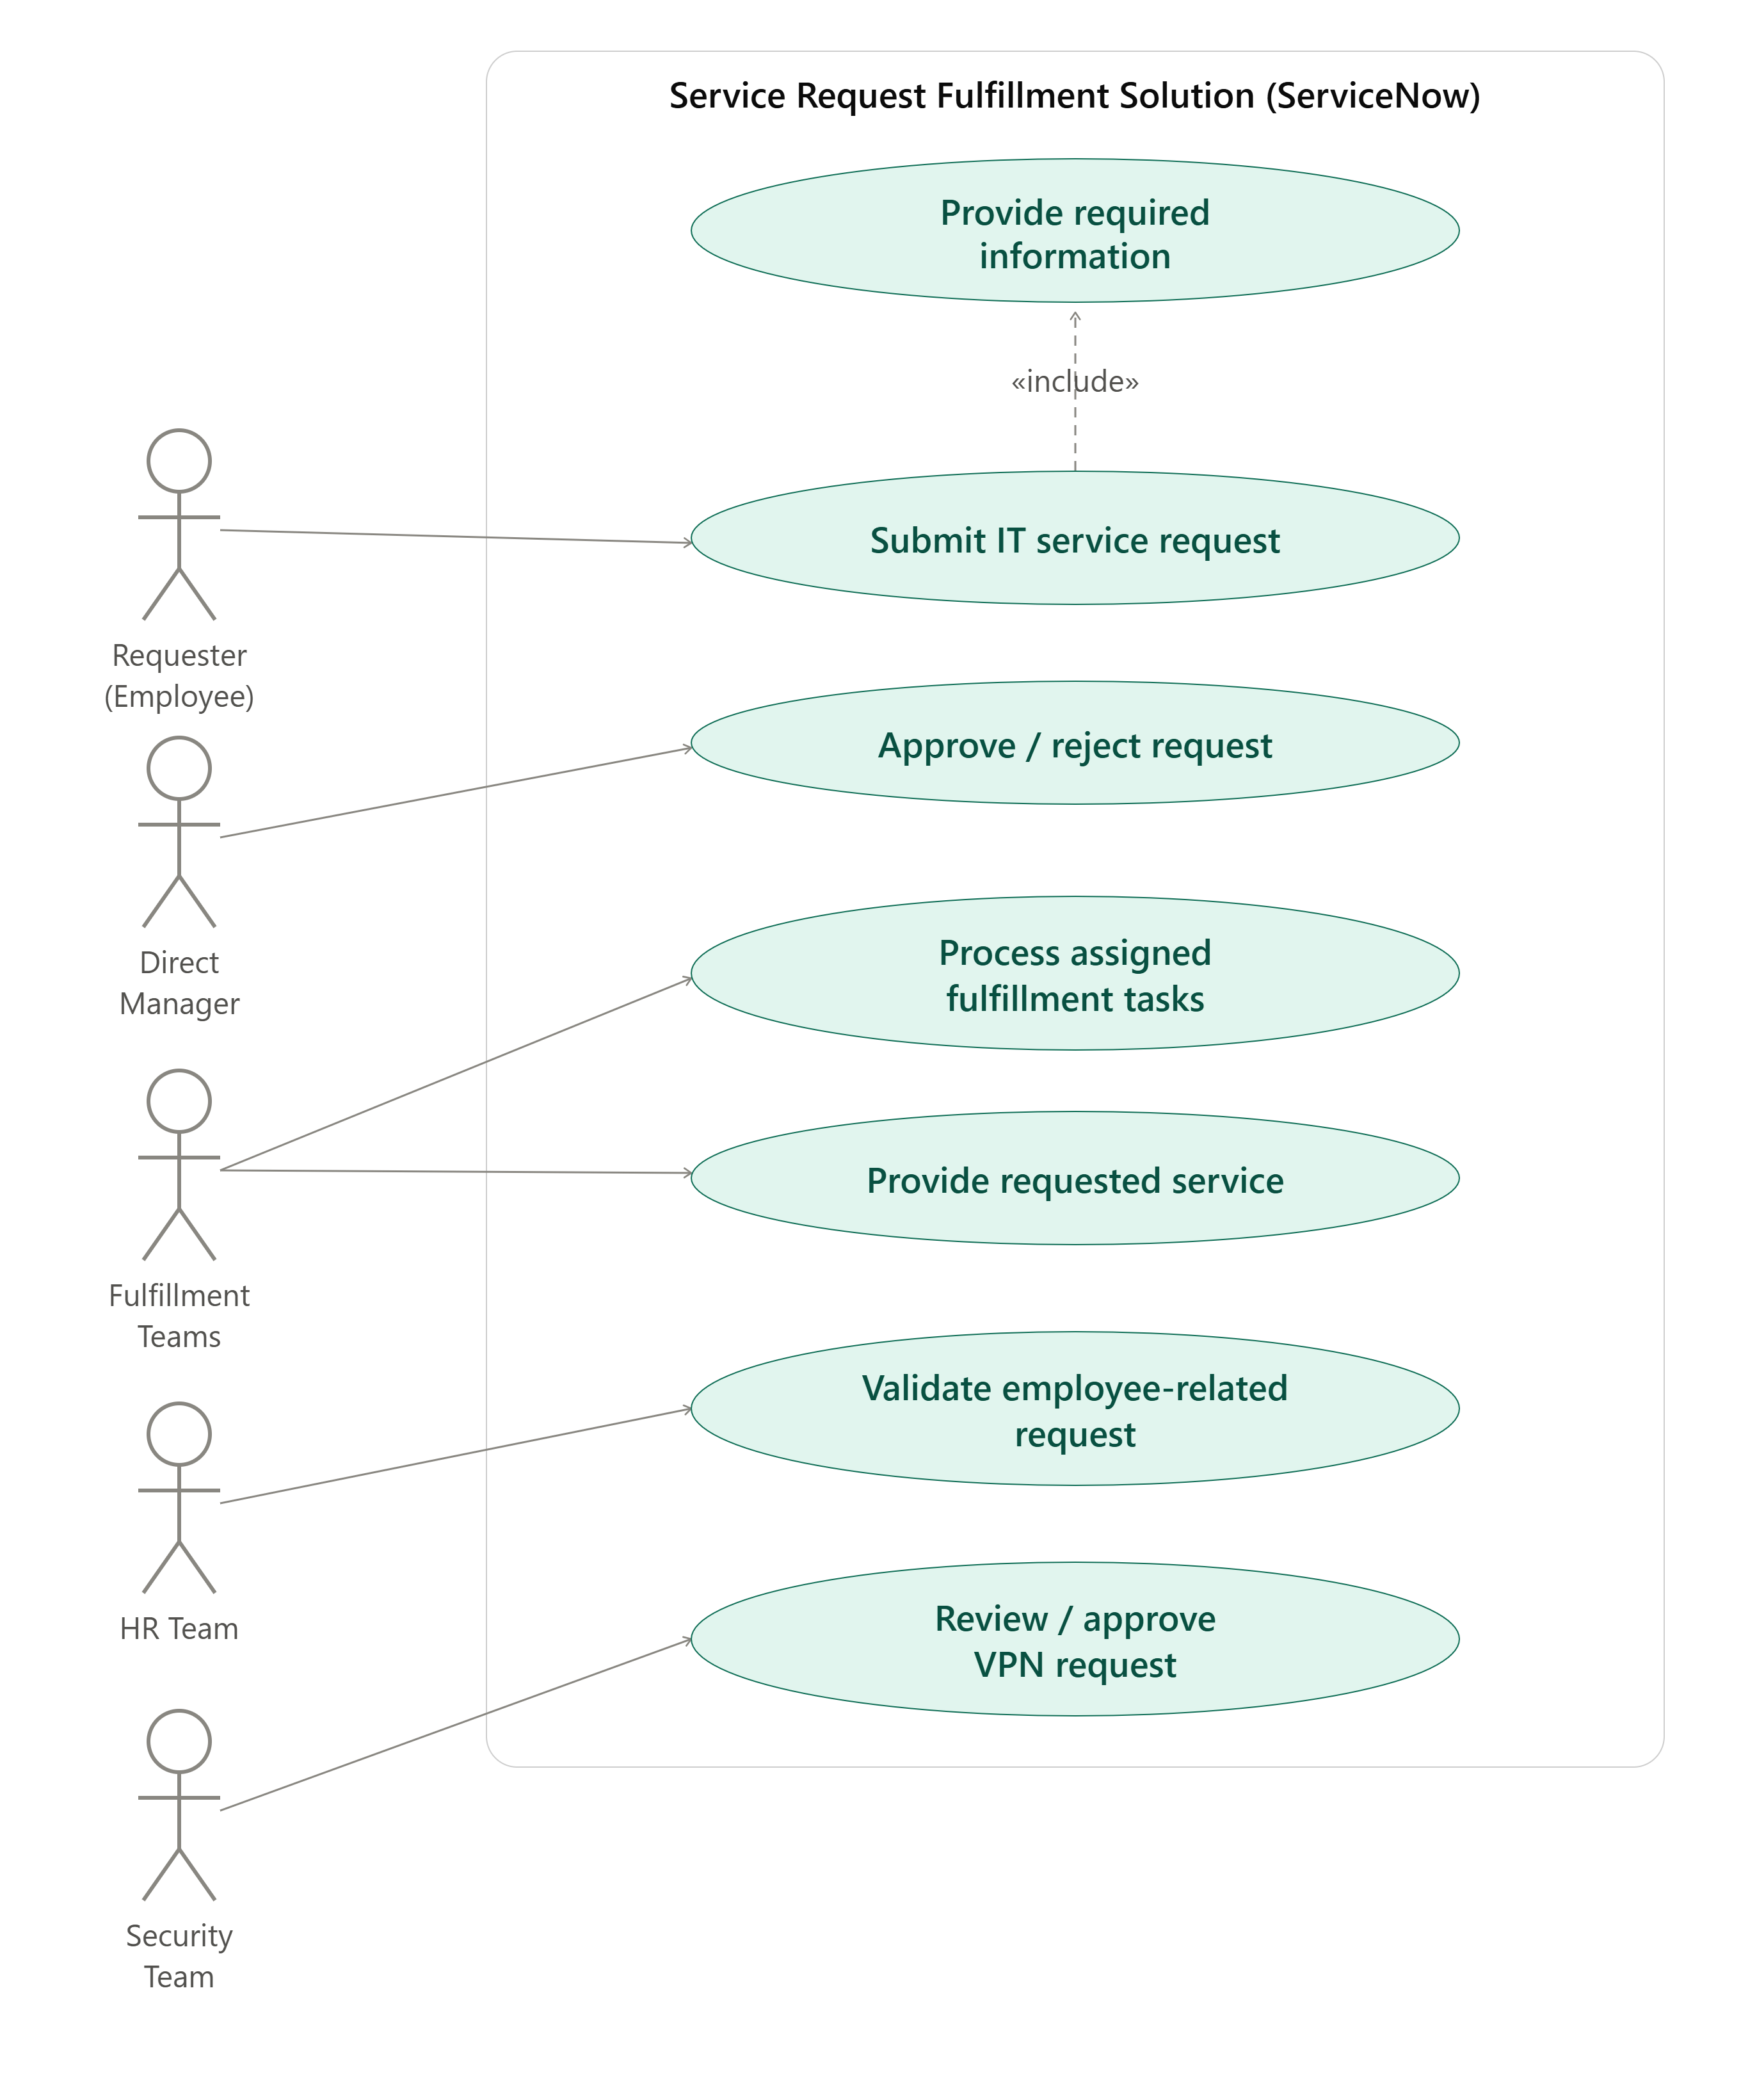
\includegraphics[width=0.75\textwidth]{service_request_use_case_diagram.png}
    \caption{Use Case Diagram of the Service Request Fulfillment Solution}
    \label{fig:use-case-diagram}
\end{figure}

\subsection{Service Request Requirements}
Each Catalog Item requires specific information and fulfillment conditions depending on the 
type of service requested. The requirements were analyzed to determine the information to be 
collected, the approvals to be obtained, and the fulfillment activities to be performed for 
each request.

\begin{table}[H]
    \centering
    \renewcommand{\arraystretch}{1.3}
    \begin{tabularx}{\textwidth}{|
        >{\raggedright\arraybackslash}p{3.0cm}|
        >{\raggedright\arraybackslash}p{2.4cm}|
        X|
        X|}
        \hline
        \textbf{Catalog Item} &
        \textbf{Category} &
        \textbf{Main Requirements} &
        \textbf{Fulfillment Activities} \\
        \hline

        Create User Account &
        User Management &
        User Concerned, Manager, Necessary Applications, Account Type,
        Start Date, Employee ID Number &
        AD account creation, mailbox creation, and application access \\
        \hline

        Enterprise VPN Access Request &
        Access Management &
        User Concerned, Access Type, Justification, Access Duration,
        Start Date, End Date &
        Security analysis, VPN configuration, User testing \\
        \hline

        Software Installation &
        Software Services &
        User Concerned, Software Requested, Computer, Version,
        Business Justification, Desired Date &
        License availability check, Software installation, User validation \\
        \hline

        IT Equipment Request &
        Hardware Services &
        User Concerned, Assigned Materials, Material Type, Reason,
        Cost Center, Quantity, Desired Date &
        Stock check, Equipment preparation, Delivery \\
        \hline

        Reset Password &
        Self Service &
        User Concerned, Application Concerned, Is Urgent, Reason &
        Password reset \\
        \hline

    \end{tabularx}
    \caption{Main Requirements of the Catalog Items}
    \label{tab:catalog-item-requirements}
\end{table}


The analysis of these requirements provided the basis for defining the
specific forms, approval processes, conditions, and fulfillment tasks
associated with each Catalog Item. The resulting workflows were designed to
adapt the processing of each request according to its specific requirements.

\subsection{Request and Approval Workflows}

The analysis of the five Catalog Items showed that each request follows a
specific fulfillment workflow based on its requirements and approval
conditions. Although the workflows share common stages, such as request
submission, approval, task fulfillment, and closure, each service includes
specific conditions and activities.

The main workflow characteristics of the five Catalog Items are summarized in
Table~\ref{tab:request-workflows}.

\begin{table}[H]
    \centering
    \renewcommand{\arraystretch}{1.3}
    \begin{tabularx}{\textwidth}{|
        >{\raggedright\arraybackslash}p{3.2cm}|
        >{\raggedright\arraybackslash}p{3.4cm}|
        X|}
        \hline
        \textbf{Catalog Item} &
        \textbf{Approval Process} &
        \textbf{Main Workflow Activities} \\
        \hline

        Create User Account &
        Manager approval followed by HR approval &
        Determine account type and priority, create AD account,
        create mailbox, and assign application access when required. \\
        \hline

        Enterprise VPN Access Request &
        Manager approval followed by Security Team approval &
        Determine priority, perform security analysis, configure VPN,
        and conduct user testing. \\
        \hline

        Software Installation &
        Manager approval followed by user validation &
        Check license requirement and availability, install the software,
        obtain user validation, and close the request. \\
        \hline

        IT Equipment Request &
        Manager approval &
        Check equipment availability, determine priority, prepare and
        deliver the equipment, and update the CMDB. \\
        \hline

        Password Reset &
        No approval required &
        Determine priority according to urgency, create the password
        reset task, and close the request after completion. \\
        \hline

    \end{tabularx}
    \caption{Main Characteristics of the Request Workflows}
    \label{tab:request-workflows}
\end{table}

The functional analysis shows that the workflows cannot follow a single
standard process. Instead, each workflow adapts to the characteristics and
requirements of the requested service:

\begin{itemize}

    \item \textbf{Simple Requests:} Requests such as Password Reset do not
    require managerial approval and can proceed directly to fulfillment,
    with their priority determined according to the urgency of the request.

    \item \textbf{Requests Requiring Managerial Approval:} Requests such as
    Software Installation and IT Equipment Request require Direct Manager
    approval before the fulfillment activities can begin.

    \item \textbf{Requests Requiring Multiple Approvals:} Requests such as
    User Account Creation and Enterprise VPN Access require additional
    validation after managerial approval, involving the HR Team or Security
    Team respectively.

\end{itemize}

The workflows also include conditional paths to handle specific situations.
For example, rejected approvals result in the request being closed as
incomplete, while conditions such as account type, software license
availability, equipment stock, and request urgency can modify the subsequent
processing of a request.

This approach allows each Catalog Item to follow a controlled process adapted
to its specific requirements while maintaining a consistent overall
fulfillment structure.

\section{Solution Design}

\subsection{Proposed ServiceNow Architecture}
The proposed solution is built on the ServiceNow ITSM architecture and uses the platform's request 
management structure to organize the fulfillment of IT service requests. When a user submits a 
Catalog Item, ServiceNow creates a hierarchy of related records that supports the request throughout 
its lifecycle.

\begin{enumerate}
    \item \textbf{Request (REQ):} Represents the overall request submitted
    by the user and acts as the container for the requested services.

    \item \textbf{Requested Item (RITM):} Represents the specific Catalog Item
    requested by the user and contains the information collected through its
    request form.

    \item \textbf{Catalog Task (SCTASK):} Represents an individual fulfillment
    activity generated for the Requested Item and assigned to the appropriate
    fulfillment team.
\end{enumerate}

The RITM serves as the central element of the fulfillment process. Once it is
created, the corresponding Flow Designer workflow manages the required
conditions, approvals, and fulfillment tasks. Depending on the requested
service, one or more SCTASKs can be generated and assigned to the appropriate
teams until the request is completed.

This architecture provides a structured relationship between the user
request, the requested service, and the activities required for its
fulfillment, while supporting centralized tracking of the request lifecycle.

Figure~\ref{fig:servicenow-solution-architecture} illustrates the proposed
architecture of the Service Request Fulfillment solution.

\begin{figure}[H]
    \centering
    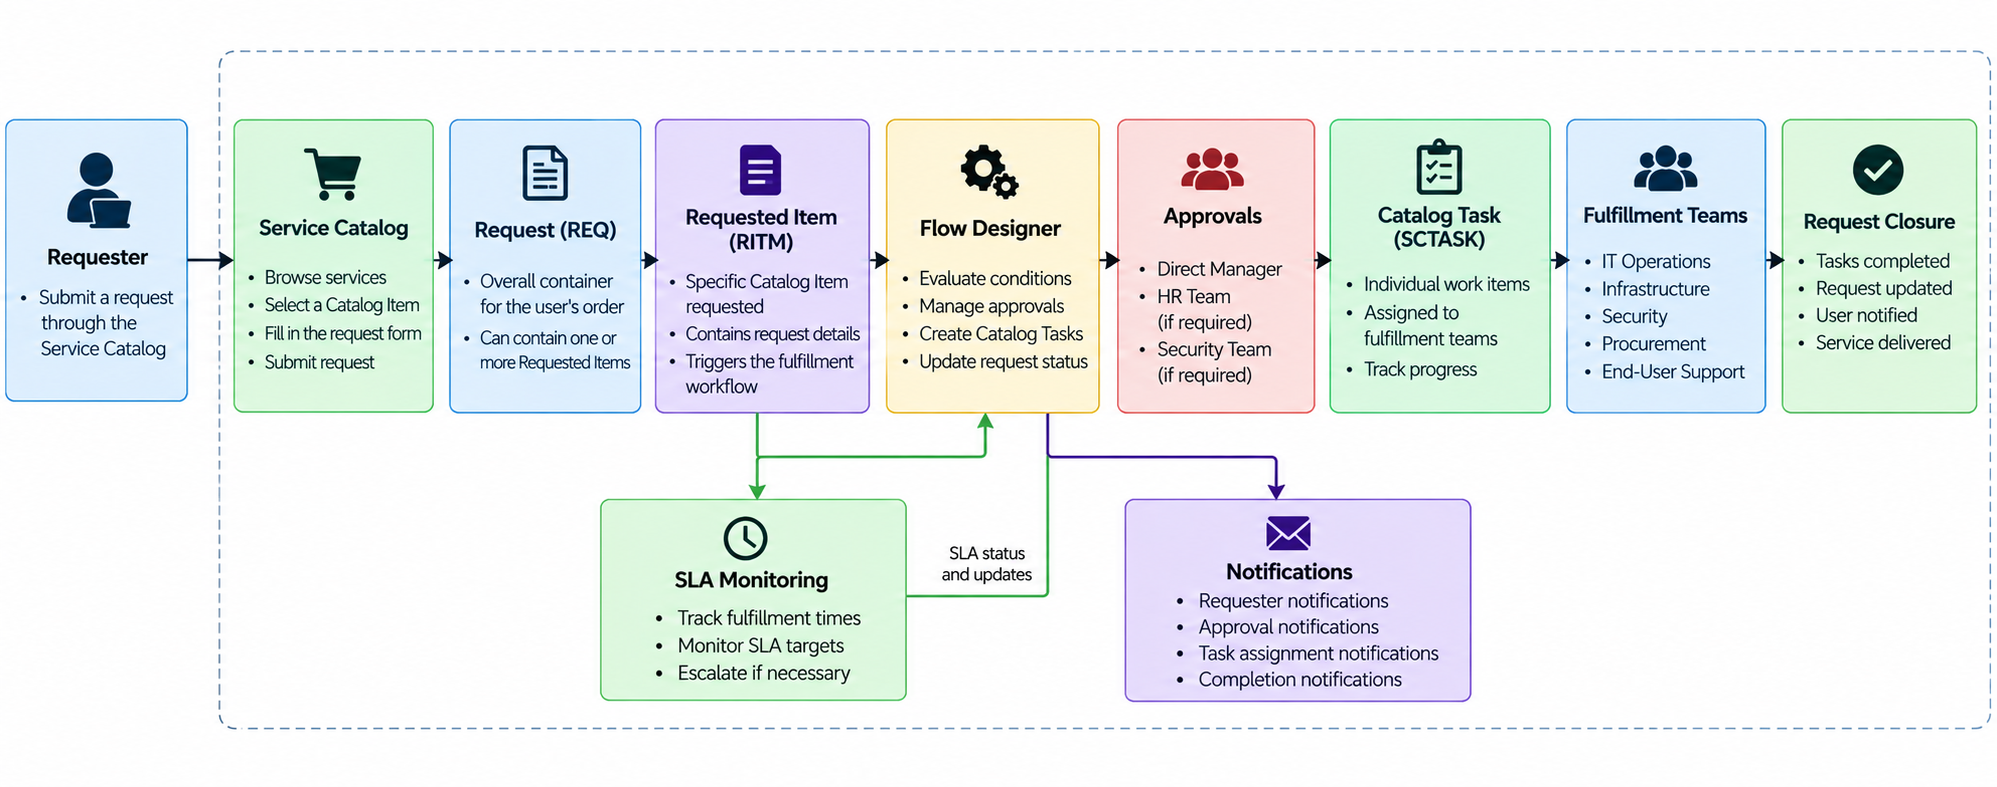
\includegraphics[width=1.10\textwidth]{servicenow_solution_architecture.png}
    \caption{Proposed Architecture of the Service Request Fulfillment Solution}
    \label{fig:servicenow-solution-architecture}
\end{figure}

\subsection{Service Catalog Structure}

The proposed Service Catalog is organized around five Catalog Items, each
corresponding to a specific type of IT service request. This structure allows
users to identify the required service easily while ensuring that each request
is associated with the appropriate information and fulfillment process.

The Catalog Items are organized into logical categories according to the type
of service they provide:

\begin{itemize}
    \item \textbf{User Management:} Create User Account
    \item \textbf{Access Management:} Enterprise VPN Access Request
    \item \textbf{Software Services:} Software Installation
    \item \textbf{Hardware Services:} IT Equipment Request
    \item \textbf{Self Service:} Reset Password
\end{itemize}

Each Catalog Item is associated with a dedicated request form containing the
variables required for its processing. The information collected through
these forms is then used by the corresponding workflow to determine the
required conditions, approvals, and fulfillment activities.

Figure~\ref{fig:service-catalog-structure} illustrates the organization of
the proposed Service Catalog.

\begin{figure}[H]
    \centering
    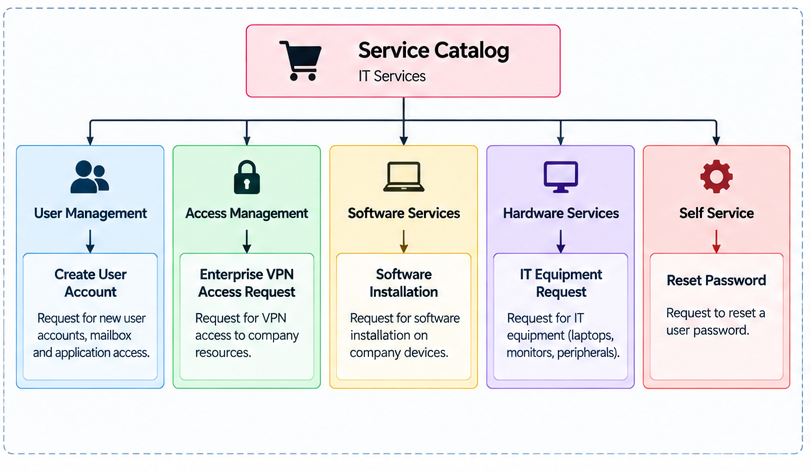
\includegraphics[width=0.9\textwidth]{service_catalog_structure.png}
    \caption{Structure of the Service Catalog}
    \label{fig:service-catalog-structure}
\end{figure}

\subsection{Request Fulfillment Workflow}

The proposed fulfillment process follows a common structure while allowing
each Catalog Item to include specific conditions and activities. Once a
request is submitted, the corresponding Requested Item is processed by the
associated workflow.

The general workflow consists of the following stages:

\begin{enumerate}
    \item \textbf{Request Submission:} The user selects a Catalog Item and
    provides the required information.

    \item \textbf{Initial Processing:} The workflow retrieves the submitted
    variables and evaluates conditions that may affect the request, such as
    account type, urgency, license requirements, or equipment availability.

    \item \textbf{Approval:} When required, the request is submitted to the
    appropriate approver. Depending on the service, this may involve the
    Direct Manager, HR Team, or Security Team.

    \item \textbf{Rejection Handling:} If an approval is rejected, the
    workflow updates the request status and closes the Requested Item as
    incomplete.

    \item \textbf{Fulfillment:} For approved requests, the workflow creates
    the required Catalog Tasks and assigns them to the appropriate
    fulfillment teams.

    \item \textbf{Validation and Closure:} Where required, the completed
    service is validated before the Requested Item is marked as complete.
\end{enumerate}

Although this general structure is shared across the solution, the workflow
branches according to the requirements of each service. For example, the
User Account Creation workflow includes Manager and HR approval, while the
Enterprise VPN Access workflow includes Manager and Security approval.
Software Installation includes a license check and user validation, whereas
IT Equipment Request includes stock verification and CMDB updating.
Password Reset follows a simpler process based primarily on request urgency.

Figure~\ref{fig:request-fulfillment-workflow} presents the general workflow
designed for the Service Request Fulfillment solution.

\begin{figure}[H]
    \centering
    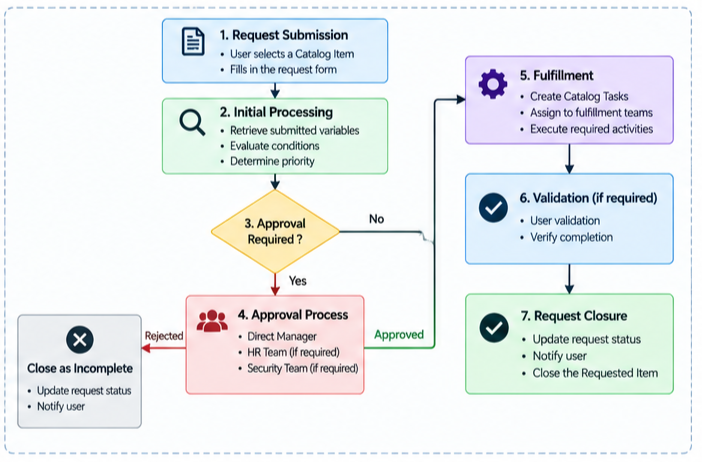
\includegraphics[width=0.95\textwidth]{request_fulfillment_workflow.png}
    \caption{General Request Fulfillment Workflow}
    \label{fig:request-fulfillment-workflow}
\end{figure}

\subsection{Request Data and Configuration Model}

The proposed solution combines ServiceNow configuration elements with the
standard request records generated during the fulfillment process. This
structure ensures that the information provided by the requester is preserved
and made available throughout the different stages of request processing.

The main elements involved are:

\begin{itemize}

    \item \textbf{Catalog Item:} Defines the service available to users and
    the information required to submit the request.

    \item \textbf{Variables:} Collect the information provided by the requester
    through the Catalog Item form. These values are used by the workflow to
    evaluate conditions and determine the required processing.

    \item \textbf{Request (REQ):} Represents the overall request submitted by
    the user and serves as a container for one or more Requested Items.

    \item \textbf{Requested Item (RITM):} Represents the specific Catalog Item
    requested and serves as the main record throughout its fulfillment
    lifecycle.

    \item \textbf{Approval Records:} Store the approval requests and decisions
    associated with the Requested Item when authorization is required.

    \item \textbf{Catalog Tasks (SCTASKs):} Represent the individual
    fulfillment activities generated from the Requested Item and assigned to
    the appropriate fulfillment teams.

\end{itemize}

The configuration elements supporting this structure include Flow Designer,
UI Policies, User Criteria, Business Rules, Service Level Agreements, and
Notifications. These elements interact with the request records to control
processing, apply conditions, manage access, monitor fulfillment times, and
communicate important updates.

Figure~\ref{fig:data-configuration-model} illustrates the relationships
between the main configuration elements and request records used in the
proposed solution.

\begin{figure}[H]
    \centering
    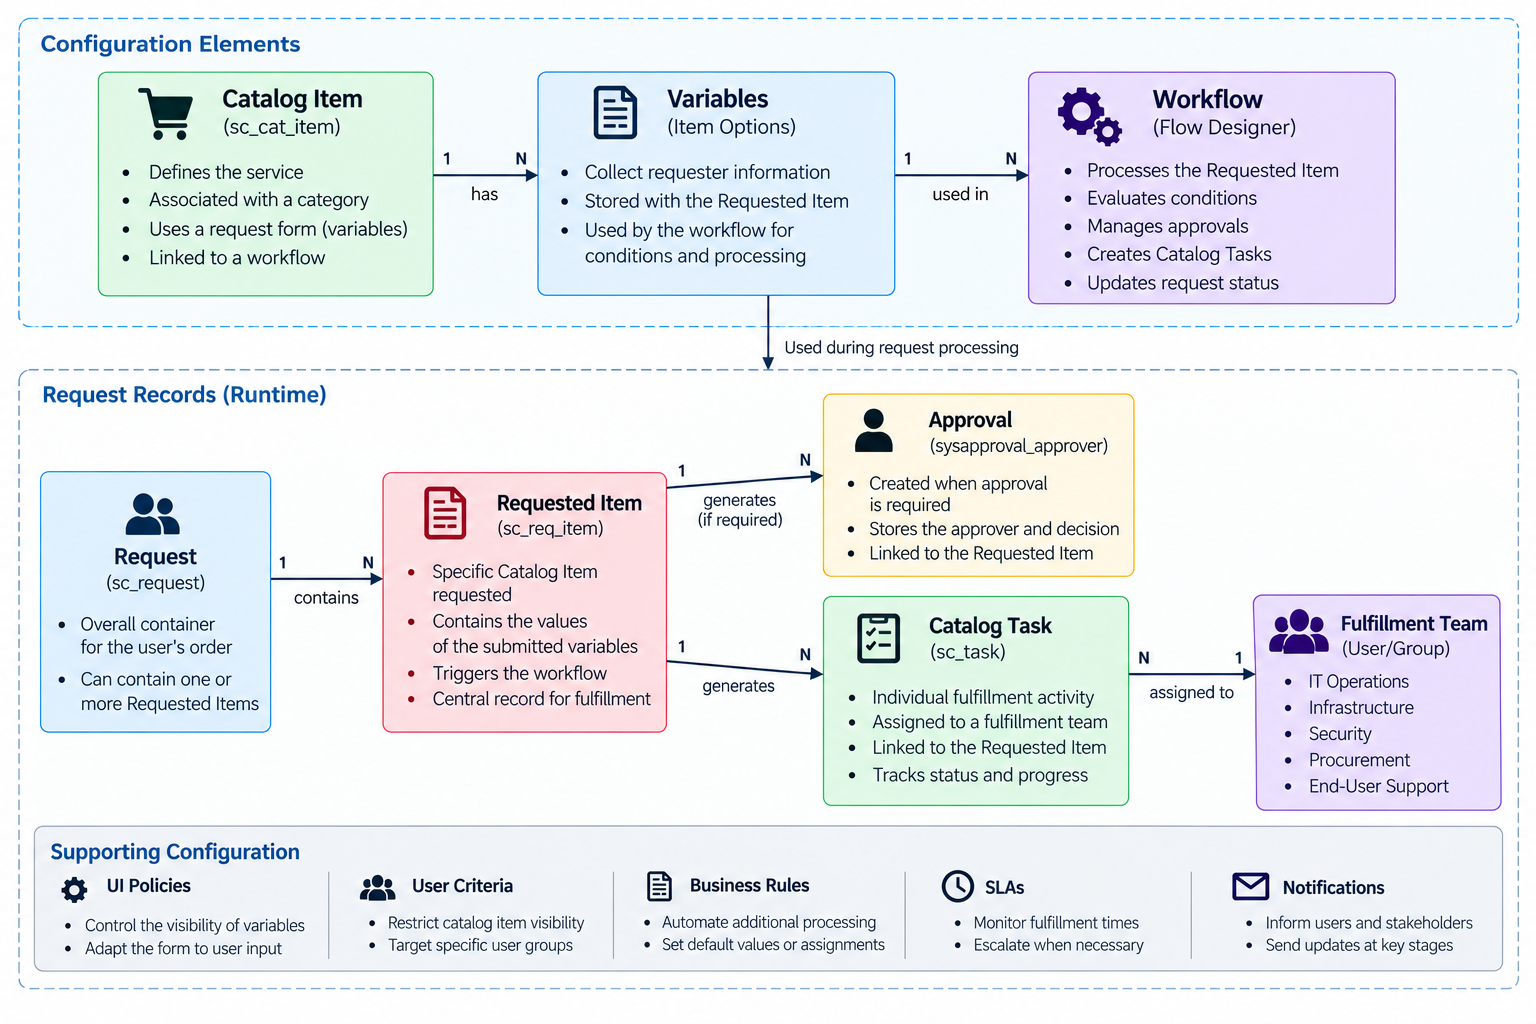
\includegraphics[width=1.0\textwidth]{data_configuration_model.png}
    \caption{Data and Configuration Model of the Solution}
    \label{fig:data-configuration-model}
\end{figure}

\section{Design of the Catalog Items}

\subsection{Create User Account}

\subsection{Enterprise VPN Access Request}

\subsection{Software Installation}

\subsection{IT Equipment Request}
\subsection{Reset Password}






































\end{document}